\documentclass[12pt]{article}
\usepackage{amssymb}
\usepackage{amsfonts}
\usepackage{amsmath}
\usepackage{float}
\usepackage{rotating}
\usepackage{pdflscape}
\usepackage{setspace}
\usepackage{threeparttable}
\usepackage{fullpage}
\usepackage{rotating}
\usepackage{booktabs}
\usepackage{array,multirow}
\usepackage{epigraph}
\usepackage[round]{natbib}
\usepackage{xcolor}
\usepackage{graphicx}
\usepackage{sectsty}
\usepackage{afterpage}
\usepackage{verbatim}
\usepackage{sverb}
\usepackage{fancyvrb}
\usepackage{soul}
\usepackage{subcaption}
\usepackage{bm}
\usepackage{titling}

%% tinytable
\usepackage{tabularray}
\usepackage{float}
\usepackage{graphicx}
\usepackage{rotating}
\usepackage[normalem]{ulem}
\UseTblrLibrary{booktabs}
\UseTblrLibrary{siunitx}
\newcommand{\tinytableTabularrayUnderline}[1]{\underline{#1}}
\newcommand{\tinytableTabularrayStrikeout}[1]{\sout{#1}}
\NewTableCommand{\tinytableDefineColor}[3]{\definecolor{#1}{#2}{#3}}

%%
\setlength\thanksmarkwidth{.5em}
\setlength\thanksmargin{-\thanksmarkwidth}
% links
\definecolor{blue}{HTML}{0188AC}
\usepackage{hyperref}
\hypersetup{colorlinks= true, allcolors = blue}

\usepackage{etoolbox} % modify commands and many other things

% Customize Figure Font and Caption Size
\renewcommand{\figurename}{\centering\normalsize{Figure}}
\renewcommand{\thefigure}{\arabic{figure}}
\newcommand{\captionfonts}{\footnotesize}
\makeatletter  % Allow the use of @ in command names
\long\def\@makecaption#1#2{%
  \vskip\abovecaptionskip
  \sbox\@tempboxa{{\captionfonts #1: #2}}%
  \ifdim \wd\@tempboxa >\hsize
    {\captionfonts #1: #2\par}
  \else
    \hbox to\hsize{\hfil\box\@tempboxa\hfil}%
  \fi
  \vskip\belowcaptionskip}
\makeatother   % Cancel the effect of \makeatletter

% Customize Table Font
\renewcommand{\tablename}{\centering\normalsize{Table}}
\renewcommand{\thetable}{\arabic{table}}

% redefine enumerate env for closer spacing
\renewenvironment{enumerate}%
  {\begin{list}{\arabic{enumi}.}%
     {\topsep=0in\itemsep=0in\parsep=0in\partopsep=0in\usecounter{enumi}}%
   }{\end{list}}

\newlength{\Oldarrayrulewidth}
\newcommand{\Cline}[2]{%
  \noalign{\global\setlength{\Oldarrayrulewidth}{\arrayrulewidth}}%
  \noalign{\global\setlength{\arrayrulewidth}{#1}}\cline{#2}%
  \noalign{\global\setlength{\arrayrulewidth}{\Oldarrayrulewidth}}}

\renewcommand{\baselinestretch}{1.5}

\textwidth = 6.5 in
\textheight = 8.8 in
\oddsidemargin = 0.0in
\evensidemargin = 0.0in
\topmargin = 0.0 in
\headheight = 0.2 in
\headsep = 0.0 in
\parskip = 0.05in
\parindent = 0.25in

\usepackage[compact]{titlesec}
\titlespacing{\section}{0pt}{*0}{*0}
\titlespacing{\subsection}{0pt}{*0}{*0}
\titlespacing{\subsubsection}{0pt}{*0}{*0}

\renewcommand{\thesubfigure}{\Alph{subfigure}}

\sectionfont{\rmfamily\normalsize\bf}
\subsectionfont{\rmfamily\it\normalsize}
\subsubsectionfont{\rmfamily\it\normalsize}

% Set your name here
\def\emailkyle{\tt{\color{blue}kbutts@uark.edu}}
\def\emailtaylor{\tt{\color{blue}taylor.jaworski@colorado.edu}}
\def\emailcarl{\tt{\color{blue}ckitchens@fsu.edu}}

% Set "thanks" indent
\makeatletter
\patchcmd\maketitle{\@makefntext}{\@@@ddt}{}{}
\patchcmd\maketitle{\rlap}{\mbox}{}{}
\makeatother

% Set footnote indent
\makeatletter
\newlength{\myFootnoteWidth}
\newlength{\myFootnoteLabel}
\setlength{\myFootnoteLabel}{.6em}%  <-- can be changed to any valid value
\renewcommand{\@makefntext}[1]{%
  \setlength{\myFootnoteWidth}{\columnwidth}%
  \addtolength{\myFootnoteWidth}{-\myFootnoteLabel}%
  \noindent\makebox[\myFootnoteLabel][r]{\@makefnmark\ }%
  \parbox[ht]{\myFootnoteWidth}{#1}%
}
\makeatother

% Fix \input with tables
% \input fails when \\ is at end of external .tex file
\makeatletter
\let\input\@@input
\makeatother

\usepackage{tikz,pgfplots}
\pgfplotsset{compat=1.17}
\usepackage{adjustbox}

% Commands for leaving comments \kyle{...}
\newtoggle{INCLUDECOMMENTS}
\toggletrue{INCLUDECOMMENTS}
% \togglefalse{INCLUDECOMMENTS}

\newcommand{\taylor}[1]{\iftoggle{INCLUDECOMMENTS}{{\color{magenta}\textbf{Taylor:} #1}}{}}
\newcommand{\kyle}[1]{\iftoggle{INCLUDECOMMENTS}{{\color{magenta}\textbf{Kyle:} #1}}{}}
\newcommand{\carl}[1]{\iftoggle{INCLUDECOMMENTS}{{\color{magenta}\textbf{Carl:} #1}}{}}


\begin{document}  
\begin{titlepage}

\title{\singlespacing {\LARGE The Urban Wage Premium in Historical Perspective}\thanks{We thank Rick Mansfield, Steve Ross, Allison Shertzer, Alex Whalley, and participants at the 2023 North American Urban Economics Association meetings (Toronto), 2023 Southern Economic Association meetings (New Orleans), and the 2025 European Urban Economic Association meetings (Berlin) for helpful comments.}}
\author{%
  \large Kyle Butts\thanks{University of Arkansas, Department of Economics, ({\emailkyle})}
  \and
  \large Taylor Jaworski\thanks{CU-Boulder, Department of Economics, and NBER ({\emailtaylor})}  
  \and
  \large Carl T.
  Kitchens\thanks{Florida State, Department of Economics, and NBER ({\emailcarl})}  
}
\date{\large \today}

\maketitle

\begin{singlespacing}
\begin{abstract}\noindent
We estimate the urban wage premium in the United States from 1940 to 2010. Drawing on advances in the literature on selection on unobservables, we show how to control for heterogeneity in the characteristics of individuals that sort into cities. Estimates from naive comparisons of individuals living in urban versus rural areas overstate the urban wage premium. We find that the premium is highest in the middle of the twentieth century relative to the early in twenty-first century. Overall, the urban wage premium is decreasing and a larger fraction is explained by sorting across our sample period.

\vspace{1em}
\noindent
\textbf{Keywords:} Urban Wage Premium, History of Cities, Agglomeration Economics
\end{abstract}
\end{singlespacing}

\thispagestyle{empty}

\end{titlepage}


%%%%%%%%%%%%%%%%%%%%%%%%%%%%%%%%%%%%%%%%%%%%%%%%%%%%%%%%%%%
\section{Introduction}
%%%%%%%%%%%%%%%%%%%%%%%%%%%%%%%%%%%%%%%%%%%%%%%%%%%%%%%%%%%

% The average US worker living in an urban area in 2010 earned 35 percent more than their non-urban counterparts.\footnote{
% Based on 2010 ACS estimates of average annual wage for individuals living in MSAs and outside of MSAs for individuals in the labor force, report non-negative wage income, and are not missing wage income data.} 
% This pattern of higher average wages in cities holds across the globe and throughout the past century \citep*{Boustan_Bunten_Hearey_2013, carlsen2016education, ahlfeldt2019economic, glaeser2022can, eliasson2023urban}.
% While the premium earned by workers has remained consistent, the role of cities in the economy has changed across time and space.
% US cities have undergone a large structural transformation from industrial bases in the middle of the twentieth century to modern service-sector focusing in finance, technology, and professional services \citep*{glaeser2001consumer,glaeser2003urban,shapiro2006smart, diamond2021spatial,connor2024frontier}.

% The fact that wages are higher in cities cannot be interpreted as the causal effect of cities due to the potential for non-random sorting into cities based on preferences, skills, or productivity.\footnote{
% For example, positive selection of firms may come from more productive firms paying higher wages, and only high-productivity firms locate and survive in cities where larger markets induce tougher competition.} 
% Is the difference driven by increased productivity stemming from agglomeration economies or high-ability workers sorting into urban areas \citep*[e.g.][]{behrens2014productive,moretti2011handbook,puga2010magnitude}?
% Empirical evidence from the last 30 years has found a large portion of the observed wage premium is driven by non-random sorting, but there is still an apparent causal effect of urban status.
% Our paper asks how the urban wage premium has changed throughout the second half of the twentieth century and to what extent this is due to the role of selection versus the causal effect of living in cities.\footnote{Previous research for the United States shows that the observed raw differences in wages between urban and non-urban workers was around 35 percent in 1940, decreasing by one-third to one half in 1980 to 20-25 percent, and increasing again to 35 percent by 2010 \citep*{Boustan_Bunten_Hearey_2013}.}

\kyle{I really like the first two paragraphs, but I think it works better like this. Above is the original version so we can restore if y'all disagree}

The average US worker living in an urban area in 2010 earned 35 percent more than their non-urban counterparts.\footnote{
Based on 2010 ACS estimates of average annual wage for individuals living in MSAs and outside of MSAs for individuals in the labor force, report non-negative wage income, and are not missing wage income data.} 
This pattern of higher average wages in cities holds across the globe and throughout the past century \citep*{Boustan_Bunten_Hearey_2013, carlsen2016education, ahlfeldt2019economic, glaeser2022can, eliasson2023urban}.
The fact that wages are higher in cities cannot be interpreted as the causal effect of cities due to the potential for non-random sorting into cities based on preferences, skills, or productivity.\footnote{
For example, positive selection of firms may come from more productive firms paying higher wages, and only high-productivity firms locate and survive in cities where larger markets induce tougher competition.} 
Is the difference driven by increased productivity stemming from agglomeration economies or high-ability workers sorting into urban areas \citep*[e.g.][]{behrens2014productive,moretti2011handbook,puga2010magnitude}?
Empirical evidence from the last 30 years has found a large portion of the observed wage premium is driven by non-random sorting, but there is still an apparent causal effect of urban status.

While the premium earned by workers has remained consistent, the role of cities in the economy has changed across time and space.
US cities have undergone a large structural transformation from industrial bases in the middle of the twentieth century to modern service-sector focusing in finance, technology, and professional services \citep*{glaeser2001consumer,glaeser2003urban,shapiro2006smart, diamond2021spatial,connor2024frontier}.
Our paper asks how the urban wage premium has changed throughout the second half of the twentieth century and to what extent this is due to the role of selection versus the causal effect of living in cities.\footnote{Previous research for the United States shows that the observed raw differences in wages between urban and non-urban workers was around 35 percent in 1940, decreasing by one-third to one half in 1980 to 20-25 percent, and increasing again to 35 percent by 2010 \citep*{Boustan_Bunten_Hearey_2013}.}

Typically, removing the role of sorting into cities is addressed using worker-level panel data.
By comparing an individual before and after moving to a city, this method removes confounding by a worker's latent unobserved productivity. 
% Comparing the same individuals before and after moving to a city removes time-invariant confounders due to sorting of workers by unobservable characteristics (e.g., ability).
The remaining gap or subsequent wage growth between urban and rural earnings is attributed to the economic effects of density \citep*{ahlfeldt2019economic, glaeser2008cities}. 
Research has explored the causes of these agglomeration effects; examples include knowledge sharing between firms, improved firm-worker matching, faster human capital accumulation, labor market pooling, or input-output linkages \citep*{BaumSnow_Pavan_2012,Combes_Duranton_Gobillon_2008,dauth2022matching, Glaeser_Mare_2001,gould2007cities,Yankow_2006,adenbaum2025there,card2024location}.

Due to data limitations, the existing literature has focused on more recent decades and little is known about the evolution of the urban wage premium before 1980.
The main challenge going back in time is that census data only provides a cross-sectional snapshot of who lives in cities and how much they earn, ruling out a strategy that relies on following workers over time.
In this paper, we show how to use readily available census data to estimate the urban wage premium while controlling for observed individual characteristics as well as unobserved characteristics following the approach in \citet*{altonji2018estimating}.

The starting point is the standard model of urban location choice \citep*{roback1982wages, bayer2007unified, bayer2016dynamic}. 
Workers vary in their willingness to pay for location-specific amenities based on their observable and, importantly, \emph{unobservable} characteristics.
Because of differences in willingness-to-pay, location-specific averages of observable characteristics vary based on the underlying amenities of a location. 
Similarly, the averages of unobservable characteristics vary because of  location-specific amenities. 
If the amenities driving both observable and unobservable sorting are the same, \citet{altonji2018estimating} show that controlling for observable location-specific averages is sufficient to control for unobservable averages.
This approach allows us to address sorting when estimating the historical urban wage premium without requiring individual-level longitudinal data.

We estimate the urban wage premium from 1940 to 2010.\footnote{We use only repeated cross-sections from the US decennial censuses and American Community Survey beginning in 1940 when information on wage income was first reported.}
First, focusing on the period since 1980, where we can make direct comparisons to the existing literature, we document an urban wage premium starting at 7.5 percent in 1980 and declining to around 5 percent in the following decades.
The estimates are consistent with the results reported in \citet*{Glaeser_Mare_2001}, \cite*{Yankow_2006}, and \citet*{BaumSnow_Pavan_2012}, and provide support that our approach addresses the key identification concern related to sorting.
Second, for the earlier decades, we estimate an urban wage premium of 11.9 percent in 1940, 15.2 percent in 1950, 12.7 percent in 1960, and 8.9 percent in 1970. 

Our results suggest that agglomeration forces were relatively more important prior to 1980, although sorting still drives a large portion of the observed premium between 1940 and 1980.
Moreover, the pattern we document is consistent with several well-documented trends in the literature. 
The increasing role of sorting fits the decision of highly educated workers to locate in cities \citep*{costa2000power,shapiro2006smart, moretti2013real, Diamond_2016}. 
Although raw differences in wages have been increasing, our results suggest that this is substantially a compositional effect rather than growth in the causal premium. 
The decreasing wage premium is also related to structural changes in manufacturing after 1950 \citep*{dumais2002geographic, glaeser2010did}. 
Historically, cities were manufacturing hubs with large agglomeration forces which enhanced worker's productivity. 
The shift away from manufacturing in cities could be a driver of the decrease in the causal wage premium. 

While urban workers may have higher wages, they also face larger housing costs, and therefore the real benefit of urban status after adjusting for housing costs may be smaller.
We calculate a wage measure that adjusts for housing costs following \citet{ganong2017has}.
Adjusting for housing prices significantly decreases the raw wage premium to around 18 percent in recent years. 
The decline is smallest around 1970 with around a 5 percentage point decline, and larger at the beginning and end of our sample with around 15 percentage point decline. 
However, our causal estimates are qualitatively similar.
There is a small decrease in 1940 and 1950, but otherwise our estimates remain stable. 

Given the large changes in the role of cities in the United States over the last 80 years, it is natural to ask how the benefits of urbanity have evolved over time and over space \citep*{glaeser2003rise,glaeser2004cities, glaeser2008rise,glaeser2010did}.
To answer this, we explore two dimensions of location: differences in city size and differences across regions in the US. 
We find that for those living in large urban areas with over 1 million residents, the urban wage premium is larger over the entire period, but the gap has narrowed since the 1980s. 
Given regional specialization in economic activity across the US, we estimate a separate premium for each census region over time.
We also find regional patterns that are consistent with the historical narrative regarding regional convergence and structural transformation \citep{barro1992convergence, kim1998economic, Mitchener_McLean_1999}. 
The Midwest had the largest urban wage premia in the middle of the century (around 25 percent in 1950) that could reflect agglomeration forces in manufacturing, while the premium has grown in the West since 1990 reflecting the growth of the technology sector.

Given these differences in premium across regions and the general evolution of cities from centers of industrial production to knowledge production and services, we empirically describe how the urban wage premium has evolved across occupations.
The general pattern that emerges is that workers in industrial production, construction, or transportation occupations experience declines in the urban wage premium. 
Workers in managerial positions or sales positions experienced positive and relatively stable premiums over time. 

\kyle{These two paragraphs felt a bit strange to me. I think it's more natural to motivate and preview the results one-by-one for each group. I made these changes, but the original one is below}

Second, we investigate whether workers with different characteristics by eduction, gender, race, and experience within a city, have experienced different wage premia.  
Given the concentration of highly educated workers in cities and the recent rise of the `consumer city', we ask whether there are increasing premiums for college workers. 
We estimate the urban wage premium for college versus non-college educated workers and find that the premium is higher for college-educated workers. 
Our estimate is consistent with the complementarity between skilled workers and cities emphasized by \citet{moretti2013real}. 

There were also sharp changes in female labor participation throughout the twentieth century, raising the question of whether similar patterns emerge for women \citep{goldin1990understanding}. 
For female workers, we estimate a similar pattern, the wage premium falls between 1940 and 1990, and then rises. 
However, the female specific urban wage premium is always higher than the premium estimated on our primary sample of male workers. 
Importantly, individual characteristics explain a larger share of the gap over time, consistent with work on the changing selection of women into the labor force. 

Beginning in the 1910s and continuing through the 1970s, Black workers migrated from rural areas in the South to urban areas across the country, with a large share moving to industrial cities in the North. 
This migration raises questions about the changing urban premium for Black workers \citep{boustan2009competition, collins2021great, derenoncourt2022can}. 
When comparing the premium for Black and white workers, the premium is no smaller than for white workers, and is particularly larger between 1950 and 1970, which is in line with the timing of the Great Migration \citep{boustan2016competition,derenoncourt2022can}.

We also consider the role of experience within cities and the urban wage growth premium as documented by \citet{BaumSnow_Pavan_2012}. 
To better understand wage growth dynamics, we estimate separate regressions for older and younger workers, assuming that the former have more years of urban experience, which should be associated with larger wage premia.
Regarding wage growth, we find that older workers have higher premia in most years, but the gap decreases over time.

% Second, we investigate whether workers with different characteristics by eduction, gender, race, and experience within a city, have experienced different wage premia.  
% Given the concentration of highly educated workers in cities and the increasing consumption in cities, we ask whether there are increasing premiums for college workers. 
% There were also sharp changes in female labor participation throughout the twentieth century, raising the question of whether similar patterns emerge for women \citep{goldin1990understanding}. 
% Beginning in the 1910s and continuing through the 1970s, Black workers migrated from rural areas in the South to urban areas across the country, with a large share moving to industrial cities in the North. 
% This migration raises questions about the changing urban premium for Black workers \citep{boustan2009competition, collins2021great, derenoncourt2022can}. 
% We also consider the role of experience within cities and the urban wage growth premium as documented by \citet{BaumSnow_Pavan_2012}. 
% To better understand wage growth dynamics, we estimate separate regressions for older and younger workers, assuming that the former have more years of urban experience, which should be associated with larger wage premia.

% We estimate the urban wage premium for college versus non-college educated workers and find that the premium is higher for college-educated workers. 
% Our estimate is consistent with the complementarity between skilled workers and cities emphasized by \citet{moretti2013real}. 
% For female workers, we estimate a similar pattern, the wage premium falls between 1940 and 1990, and then rises. 
% However, the female specific urban wage premium is always higher than the premium estimated on our primary sample of male workers. 
% Importantly, individual characteristics explain a larger share of the gap over time, consistent with work on the changing selection of women into the labor force. 
% When comparing the premium for Black and white workers, the premium is no smaller than for white workers, and is particularly larger between 1950 and 1970, which is in line with the timing of the Great Migration \citep{boustan2016competition,derenoncourt2022can}.
% Regarding wage growth, we find that older workers have higher premia in most years, but the gap decreases over time.

Overall, this paper highlights a novel approach to estimating the urban wage premium using widely available data. 
Our application of \cite{altonji2018estimating} allows us to provide estimates for a period not previously considered in the literature.
The results show a decreasing urban wage premium over time and that the importance of sorting into cities began relatively early in the twentieth century.
Importantly, we document that sorting into cities has been prevalent throughout much of the twentieth century and the highly noted widening after 1980 looks less dramatic in the historical context.  

%%%%%%%%%%%%%%%%%%%%%%%%%%%%%%%%%%%%%%%%%%%%%%%%%%%%%%%%%%%%%%%%%%%%%%%%%%%%%%%%
\section{Data and Summary Statistics}\label{sec:data}
%%%%%%%%%%%%%%%%%%%%%%%%%%%%%%%%%%%%%%%%%%%%%%%%%%%%%%%%%%%%%%%%%%%%%%%%%%%%%%%%

In this section, we describe the data we use to estimate the urban wage premium and key empirical patterns regarding the changes in urbanization, education, and the urban versus non-urban wage difference in the second half of the twentieth century.
First, we draw on publicly available data covering the period between 1940 and 2010 \citep*{ruggles2022full, ruggles2022census}.
For 1940, we use the complete count of the US Census to measure the average earnings per worker for wage earners.\footnote{In the 1940 Census wages are only reported for those working for another individual or firm. Thus, there are large differences in self employment between urban and rural-farm areas. For example, only 10.8 percent of urban workers report self employment, whereas 49.7 percent of rural-farm workers (an additional 11.1 percent are unpaid family labor) \citep{census1940pop}.}
For 1960 and 1970, we use the 5 percent samples of the census.
For 1950, 1980, 1990, and 2000, we draw on the 1 percent samples of the census.
Finally, for 2010, we use the American Community Survey.
We use person weights to calculate summary statistics and estimate regressions. 

In each year, we restrict the data to include adults living in the continental US between the ages of 25 and 65. 
Since our focus is on the wage premium, we follow the wage premium literature and restrict the sample to workers who report being employed for at least 26 weeks in the sample year.\footnote{About 80\% of our observations work the entire year and results are nearly identical when focusing just on these workers (Figure \ref{fig:premium_full_time_employees}).}
We focus on male workers since the role of women in the workforce changes over this time \citep{goldin1990understanding}. 
Including female workers in our main estimates would confound changes in the urban wage premium and changes in female labor force participation. 
In section \ref{sec:female_wage_premium}, we explore the wage premium for women. 

To construct average weekly earnings, we follow \citet{goldin1992great} and divide the reported total income by the number of weeks worked in the survey year.\footnote{For individuals earning the top income code, we set income to be the lower top income cutoff multiplied by $1.4$ following \citet{goldin1992great} These cutoffs are reported in the IPUMS documentation for the \texttt{INCWAGE} variable. In 2015 dollars, the cutoffs are \$84,500 for 1940, \$99,2000 for 1950, \$199,500 for 1960, \$309,000 for 1970, and \$225,000 for 1980. Afterward, IPUMS reports income as the median wage above that year's cutoff. Results are robust to dropping all individuals earning the top income code.} 
We then convert all earnings to 2015 dollars using the Consumer Price Index.
Since housing costs are higher in urban areas, we construct a measure of ``real wages'' following \citet{ganong2017has}. 
To do so, we use either (i) five percent of the reported housing value or twelve times the reported monthly rent and divide by 48 to get the weekly housing costs.\footnote{We windsorize our measuring of housing costs at the 1st and 99th percentiles.}
To estimate the net-of-housing-costs wages, we subtract the estimated weekly housing cost from the weekly wages.\footnote{Since 1950 does not have microdata on rent, we use the average rent from the Census tables.} 

In addition to wages, across all samples, consistent information is available on whether the individual is living in an urban area, age, educational attainment, and race.
We use this information to construct the individual- and group-level controls for our empirical analysis.
In our framework, workers are choosing over a set of locations which we define as the set of Metropolitan Statistical Areas (MSA). 
For non-urban locations, we define them as each state's non-MSA counties.
% We assign workers to a city based on the Metropolitan Statistical Area (MSA) in which they reside; workers not living in a city are assigned to their state of residence. 
For assigning workers to a specific location, we use their county of residence and the Census Bureau's Historical Delineation Files of MSAs.\footnote{For 1940, we use the 1950 delineation.} 

We use this data to document the raw observed difference between urban and rural wages to match the previous literature \citep*{moretti2013real,Boustan_Bunten_Hearey_2013}.\footnote{Table \ref{tab:summ} reports summary statistics for each year between 1940 and 2010.}
The urban wage gap started at 31.3 percent in 1940 and declined sharply through 1980.
Beginning in 1980, the urban wage gap increased until 2000 where it reached nearly the same level as reported in 1940.
In addition, over this period, the fraction of people living in urban areas increased from  66 percent in 1940 to nearly 80 in 2010.
To highlight the potential role of sorting, we also calculate the fraction of the population with college degree in each year and differences in this share across urban and non-urban areas.
The share of the population with a college degree increased over time and the share increases for both urban and rural areas; however, the share rises faster in cities.
Together, these trends highlight that cities have become more populated and more-educated relative to rural areas, which suggests increased sorting \citep{glaeser2003rise, diamond2021spatial}.

The geography of high-wage urban centers has also changed over time.\footnote{Table \ref{tab:top} reports the ten urban areas with the highest urban wage differences in 1940 and 2010.}
In particular, we calculate the difference in the average log wage in an urban and non-urban area.
While several of the cities are among the highest paying in both 1940 and in 2010 (i.e., San Francisco, Washington, DC, San Jose, Seattle), centers of manufacturing in the industrial North and Midwest (i.e., Flint, MI, Detroit, MI, Lansing, MI, Chicago, IL, Rochester, NY) have lost their prominence in favor of cities closely associated with high-tech manufacturing.
This descriptive pattern reflects the combination of several changes in the US economy since 1940.
In the remainder of the paper, we develop an empirical strategy to quantify and better understand changes in the urban wage premium over time and the relative importance of the causal effect of cities (i.e., due to agglomeration) versus sorting. 

%%%%%%%%%%%%%%%%%%%%%%%%%%%%%%%%%%%%%%%%%%%%%%%%%%%%%%%%%%%
\section{The Naive Urban Wage Premium}
%%%%%%%%%%%%%%%%%%%%%%%%%%%%%%%%%%%%%%%%%%%%%%%%%%%%%%%%%%%

We begin by estimating the urban-rural wage difference in a simple regression framework.
We follow the literature by adding individual-level covariates to address sorting into urban locations.
In particular, we estimate the following equation separately for each year:
\begin{equation}\label{eq:controls}
    \log(\text{wage}_i) = \beta_0 + \beta_1 \text{urban}_i + \bm{X}_{i} \delta + \varepsilon_i,
\end{equation}
where $\text{wage}_i$ is average weekly earnings and $\bm{X}_i$ is a set of control variables consisting of indicator variables for five-year age bins, educational attainment dummy variables, and an indicator for race (white versus non-white).\footnote{
We are limited in our control variables because we want these to remain constant across census years.}

Our variable of interest is $\text{urban}_i$ which for the purpose of our study we define as residing in a Metropolitan Statistical Area.\footnote{
Note that the number of MSAs changes over our sample period.
This raises a concern that our estimates may reflect a change in the composition of MSAs.
As an alternative to our main approach, we also re-estimate equation \eqref{eq:AM} with a fixed sample of MSAs based on their 1940 designations and drop observations from MSAs designated after 1940 from the sample.
In Figure \ref{fig:premium_msa_in_all_yrs} we report the estimates holding the set of MSAs constant.
We obtain similar results, which suggests that the changing composition of cities does not bias our estimates.    
}
Our estimate of $\beta_1$ is the average premium in percentage terms that urban workers earn relative to non-urban workers (in figures we calculate percent using the $e^{\hat{\beta}_1} - 1$ formula).
Without controls, the coefficient reflects the mean difference in earnings between individuals living in urban and non-urban locations.
If the set of control variables fully accounts for sorting, we could interpret $\beta_1$ as the causal effect of living in an urban location on earnings.
However, there are several reasons individuals sort into cities that are not captured by their observable characteristics.
For example, individuals with certain attributes may sort to cities because they value specific consumptive amenities, such as entertainment or dining.
If these sorting patterns are correlated with productivity, $\beta_1$ would suffer from omitted variables bias.
As a result, the estimated $\beta_1$ should be interpreted as a correlation.

The results of estimating equation (\ref{eq:controls}) with and without controls are displayed in Figure \ref{fig:premium_over_time}.
The gray line with square markers reports the mean urban wage difference without any covariates.
This difference was highest in 1940 at around 35 percent and falls to a little under 25 percent by 1970.
Starting around 1980, the difference stabilizes at around 20 percent.
The gray line with circle markers reports estimates that include individual-level controls.
Adding individual-level covariates reduces the wage differential in all years.
In 1940, individual characteristics explained roughly 10 percent of the gap between non-urban and urban workers.
By 2010, differences in individual-level observables explained about 25 percent of the gap.
We use a smaller set of observable controls relative to the literature \citep[e.g.,][]{Yankow_2006,Glaeser_Mare_2001}, however the qualitative pattern is similar.

%We also show that individual characteristics explain a larger share of the urban wage differential over time.\footnote{This suggests that sorting -- despite our limited set of observables -- is increasing over time and is consistent with the raw data in Table \ref{tab:summ}. Note that the reason for the difference in estimates relative to \citet{Boustan_Bunten_Hearey_2013} who find a U-shaped pattern comes from our use of a regression framework. The method in \citet{Boustan_Bunten_Hearey_2013} estimates $ \log( \hat{\mathbb{E}}[\text{Wage} \ |\  \text{Urban} = 1] ) - \log( \hat{\mathbb{E}}[\text{Wage} \ |\ \text{Urban} = 0] )$, which differs from the regression estimate, $\hat{\beta}_1 = \hat{\mathbb{E}}[ \log(\text{Wage}) \ |\  \text{Urban} = 1] - \hat{\mathbb{E}}[ \log(\text{Wage}) \ |\  \text{Urban} = 0]$.
%The latter is a more precise estimate for average percent difference in wages.}

%%%%%%%%%%%%%%%%%%%%%%%%%%%%%%%%%%%%%%%%%%%%%%%%%%%%%%%%%%%
\section{Addressing Sorting and Selection}\label{sec:sorting}
%%%%%%%%%%%%%%%%%%%%%%%%%%%%%%%%%%%%%%%%%%%%%%%%%%%%%%%%%%%

The estimates from the previous section are potentially biased if sorting causes urban workers and non-urban workers to differ in their underlying productivities.
For example, if the movement of high-skilled workers to dense cities is driven in large part by differences in preferences for consumption amenities, then the estimated premium would measure the combination of the true premium and the compositional differences in worker productivity due to sorting for amenities.
This creates our main identification challenge: if amenities that are abundant in a city attract more productive workers, then the estimates of equation \eqref{eq:controls} will be biased upward. 
Previous work has leveraged panel data on individuals to isolate the effect of living in an urban area by observing individuals who transition across urban and non-urban locations.\footnote{Recent examples include \citet{frings2022relative}, \citet{eckert2022return}, \citet{card2024location}, and \citet{adenbaum2025there}.} 
Given the cross-sectional nature of our data, we cannot adopt these panel data methods.

Starting with the standard omitted variables bias formula, our coefficient $\hat{\beta_1}$ from equation  (\ref{eq:controls}) would be biased if people living in urban areas have different unobservable characteristics ($X_{i}^{U}$) and these characteristics are associated with productivity.
Note, we do not need to observe the unobservable characteristics at the individual level.
Instead, it is sufficient to control for \emph{location averages} of unobservables, $\bar{\bm{X}}_\ell^U$ to remove the bias.
Since we can not directly measure unobservables, we will draw on the properties of the canonical location choice model in urban economics for a solution.
As shown by \citet{altonji2018estimating}, this model yields statistics from observable data that we use to isolate the causal wage premium. 

To build intuition on the approach, consider parents deciding where to live and send their children to school. 
Some parents may have a preference for their children to attend a high quality school; this preference is unobservable in the data.
If the preference for high quality schools is correlated with the observable education level of parents, then locations with high shares of college-educated workers will tend to be locations with high quality schools. 
Therefore, under a set of formal conditions we outline below, including the average level of education or the fraction of individuals that have completed college in a location controls for the (unobserved) amenities that drive sorting. 

In the location choice model, individuals have an indirect utility function over locations $\ell$ that depends on a vector of location-specific amenities, $\bm{A}_\ell$, and the cost to live in that location, ${P}_\ell$: 
\begin{equation}
    \text{V}_{i \ell} = \bm{W}_i \bm{A}_\ell - {P}_\ell + \varepsilon_{i \ell} .
\end{equation} 
Here $\bm{W}_i$ is a vector of an individuals' willingness to pay for each amenity.\footnote{
  This multinomial model of utility is common in urban economics \citep*[e.g.][]{Kline_Moretti_2014,diamond2021spatial}.
}
To allow for rich sorting patterns, the willingness to pay parameters are assumed to be an additive function of observable characteristics $\bm{X}_i$ and unobservable characteristics $\bm{X}_i^\text{U}$ of the worker:
\begin{equation}\label{eq:loc choice sub}
    \text{V}_{i \ell} = (\bm{X}_i \bm{\Theta} + \bm{X}_i^\text{U} \bm{\Theta}^\text{U}) \bm{A}_\ell - {P}_\ell + \varepsilon_{i \ell}.
\end{equation} 
Each worker receives a set of idiosyncratic preference draws, $\varepsilon_{i \ell}$ for each location $\ell$.
As is standard in the literature, we assume the shocks $\varepsilon_{i \ell}$ are mean zero and drawn independently from $\bm{X}_i, \bm{X}_i^{\text{U}}, \bm{A}_\ell,$ and $P_\ell$. 
Workers then chose the location that maximizes their indirect utility assuming they take the amenities and prices as given.

%In this model, the previous section's urban wage premium estimates will be biased if two things are true. First, in order for sorting to occur, urban locations must differ in amenities compared to non-urban locations. Second, the unobservable characteristics that change willingness to pay for these amenities, $\bm{X}_i^\text{U}$, must also affect productivity. For example, \citet{Diamond_2016} finds that the movement of high-skilled workers into dense cities is driven in large part by differences in preferences for consumptive amenities. This creates our main identification challenge: if the kinds of amenities that are abundant in cities attract more productive workers, then the estimates of equation (\ref{eq:controls}) will be biased upwards.

Since individuals maximize their indirect utility when choosing where to live, we expect location averages of $\bm{X}_i$ and $\bm{X}_i^\text{U}$ to both be correlated with (some of) the amenities.
That is, there exists some mapping between location averages of unobservables $\bar{\bm{X}}_\ell^\text{U} \equiv \mathbb{E}\left[ \bm{X}_i^U \ \vert \ \ell(i) = \ell \right]$ and amenities $\bm{A}_\ell$, say $\bar{\bm{X}}_\ell^\text{U} = f^{\text{U}}(\bm{A}_\ell)$. 
The same logic holds for averages of observables $\bar{\bm{X}}_\ell = f(\bm{A}_\ell)$. 
Under conditions we will discuss below, we can invert the latter equation to solve for amenities $\bm{A}_\ell = f^{-1}(\bar{\bm{X}}_\ell)$.
Plugging this into the the former equation yields $\bar{\bm{X}}_\ell^{\text{U}} = f^{\text{U}}(f^{-1}(\bar{\bm{X}}_\ell))$.
Since we can construct $\bar{\bm{X}}_\ell$ from our data, if we knew $f^{\text{U}}$ and $f$, we could estimate $\bar{\bm{X}}_\ell^U$. 
The estimated $\bar{\bm{X}}_\ell^U$ would allow us to control for the effects of sorting in our regression. 

\citet{altonji2018estimating} show that under a set of conditions that we discuss below, this mapping from observable averages to unobservable averages is a \emph{linear} function, 
i.e. $f^{\text{U}}(f( \bm{X}_\ell )) = \bm{X}_{\ell} \bm{B}$ for some invertible matrix $\bm{B}$. 
This allows us to rewrite equation (\ref{eq:controls}) to include group-level averages of the individual characteristics in each location.
\begin{equation}
    \label{eq:AM}
    \log \text{wage}_i = \beta_0 + \beta_1 \text{urban}_i + \bm{X}_{i} \delta + \bar{\bm{X}}_{\ell(i)}\gamma + \varepsilon_i,
\end{equation} 
where $\bar{\bm{X}}_{\ell(i)}$ are the location-specific average of the individual characteristics in $\bm{X}_i$ and additional location-invariant characteristics.
We include as group-averages the share of white workers; share of residents in all but one of the age groups; share that are veterans; share that are married and together, married and apart, and single; and share with less than a high school degree, share with a high school degree, share with some college, share with BA degree, and share with advanced education.
We also include a measure of market access calculated as in \citet{Jaworski_Kitchens_2019}.

Our estimate $\beta_1$ now captures the causal urban wage premium since the group averages control for the sorting of individuals.
Note that by controlling for the average characteristics of a worker's neighbors, we are, in effect, controlling for peer effects on a worker's wages. 
Our estimate may, therefore, underestimate the true impact of living in a city if it mainly operates through better peer-networks. 
There are two reasons that we think alleviate this concern. 
First, recent work trying to `decompose' the wage premium does not point to peer effects as being a particularly important component, e.g. \citet{card2024location} and \citet{adenbaum2025there}.
Second, in practice our estimates in later decades match other estimates found using panel data.

Under five assumptions, we are able to exploit the above linear mapping and therefore absorb the bias due to sorting of workers.
First, preferences are given by equation \eqref{eq:loc choice sub}.
Second, $\varepsilon_{i \ell}$ are assumed to be mean zero and drawn independently from observables, unobservables, and amenities of the locations. 
Third, workers select their location taking prices and amenities as given.
The wide-spread use of these kinds of models in urban economics makes these three assumptions standard.

The final two assumptions restrict the relationships between $\bm{X}_i$, $\bm{X}_i^{\text{U}}$ and $\bm{A}_\ell$. 
The fourth assumption is we need the set of location-specific amenities that drive sorting on \emph{observable} covariates to contain \emph{all} location-specific amenities that drive sorting based on \emph{unobservable} covariates.
%As an example of where this might break down, say workers with high creative intelligence are sorting into cities based on the large amount of arts available. 
%If no observable characteristics alters the worker's willingness to pay to live in an area with arts, then the `inversion' of $\bar{\bm{X}}_i$ to $\bm{A}_\ell$ can not inform us about a location's arts amenity and therefore can not inform us about the average creative intelligence of it's workers.  
Finally, we require the mapping $f( \bar{\bm{X}}_\ell ) = \bm{A}_\ell$ to be invertible. 
This requires (i) the vector of observable characteristics used must explain the willingness to pay for a wide range of amenities and (ii) the number of observable averages we use must be larger than the number of amenities that workers chose from.

A simple way to think about these conditions is via the following infeasible regressions.
First, consider regressions of location-averages of observable characteristics on amenities:
\begin{equation}\label{eq:observables_on_amenities}
    \bar{\bm{X}}_\ell = \bm{A}_\ell \bm{\Pi} + \bm{u}_i.
\end{equation}
The coefficients $\bm{\Pi}$ provide a reduced form measure of how sorting on observables relates to amenities. 
Since $\bm{X}_\ell$ is a vector, $\bm{\Pi}$ is a matrix of coefficients. 
If a row of $\bm{\Pi}$ is equal to 0, that would imply that the given amenity is not a driver of sorting on observables (conditional on other amenities).
That would make knowledge of $\bm{X}_\ell$ uninformative about that specific amenity and would violate assumption 4.  

The inversion procedure involves solving $\bar{\bm{X}}_\ell = \bm{A}_\ell \hat{\bm{\Pi}}$ for amenities $\bm{A}_\ell$. 
For this to be possible, requires the matrix $\bm{\Pi}$ to have rank larger than the rank of $\bm{A}_\ell$. 
That is, we need more informationally distinct observable averages than the number of amenities. 
In practice many amenities are bundled together in the sense that a location high in one amenity is very likely to be high other amenities. 
\citet{Diamond_2016} provides evidence using a principal component analysis on a detailed set of amenities and documents that the effective rank s around five (with three components explaining most of the variation).
In the context of this paper, the key identifying assumptions are that our group-average variables have an effective (column) rank larger than five.
We run principal components analysis and find more than five components that explain more than 5 percent of the total variance across years.
We also merge our group-level averages with the amenities in \citet{Diamond_2016} in 2000, when we have overlap with 186 MSAs.
Regressing the amenities matrix on our group-level averages generates a matrix of coefficients that is full row-rank, providing support for the matrix inversion.

Second, consider regressions of location-averages of unobservable characteristics on amenities:
\begin{equation}\label{eq:unobservables_on_amenities}
    \bar{\bm{X}}_\ell^U = \bm{A}_\ell \bm{\Gamma} + \bm{v}_i.
\end{equation}
The columns of $\bm{\Gamma}$ must all be non-zero so that amenities are informative about \emph{every} unobservable characteristic. 
Since this assumption is based on two sets of unobservables, we can not provide direct evidence. 
The final step of our procedure would be to take the inverted amenities $\hat{\bm{A}}_\ell$ and multiply by $\hat{\bm{\Gamma}}$ to estimate $\bar{\bm{X}}_\ell^U$.
While we cannot do this directly, the logic of \citet{altonji2018estimating} is that including group-level averages serves as a control function for these unobserved amenities.

Finally, we re-estimate the model dropping each of the group averages separately.
If we have sufficiently rich group averages, then dropping a single average should not qualitatively change our point estimates. 
In appendix figure \ref{fig:leave_one_group_average_out}, we show that these estimates are quite stable.

\section{Estimates of the Causal Urban Wage Premium}

We present our main estimates of equation \eqref{eq:AM} for each year in Figure \ref{fig:causal_premium}.\footnote{
Note that he number of MSAs changes over our sample period.
This raises a concern that our estimates may reflect a change in the composition of MSAs.
As an alternative to our main approach, we also re-estimate equation \eqref{eq:AM} with a fixed sample of MSAs based on their 1940 designations and drop observations from MSAs designated after 1940 from the sample.
In Figure \ref{fig:premium_msa_in_all_yrs} we report the estimates holding the set of MSAs constant.
We obtain similar results, which suggests that the changing composition of cities does not bias our estimates.    
}
These estimates make clear that using the group-level averages of individual characteristics to control for sorting decreases the urban wage premium significantly.
Relative to the naive estimates, these results suggest that individual characteristics and sorting explain approximately 75 percent of the wage differential between urban and non-urban areas after 1980 and approximately half in earlier decades.

Focusing on the period between 1980 and 2010, when our estimates overlap those reported in the existing literature, we find an urban wage premium of approximately 5 percent in each year.
Table \ref{tbl:estimates-in-literature} presents an overview of estimates in the literature that use panel-data with individual fixed-effects.
% Our estimates closely match those in \citet*{Glaeser_Mare_2001}, who report a premium of 4.5 percent in the densest metropolitan areas.
% Our estimates also mirror those reported by \cite*{Yankow_2006}, whose fixed effects estimates range from 4.9 to 5.4 percent.
% Our estimates are also within the range of those in \citet*{BaumSnow_Pavan_2012}.
Remarkably, our estimates are closely in line with the literature that uses the `movers' design with panel data.
The overlap of our estimates for the decades since 1980 and previous estimates provides support for our approach using group-level averages to address the potential role of sorting.

Next, we turn to the period from 1940 to 1980, where the previous literature has yet to provide estimates of the urban wage premium.
In 1940, we find that the urban wage premium was approximately 13 percent.\footnote{
The estimates for 1940 may differ from the estimates in other decades for several reasons. First, the 1940 Census only reports wages for wage workers and not income for all workers. Thus, the composition of employment in 1940 may differ relative to later decades. Second, New Deal labor policies such as the National Industrial Recovery Act (NIRA) aimed at wage earners to restrict hours and raise wages may have had persistent effects after being declared unconstitutional in 1935 \citep{cole2004new,fishback2024labor}. To the extent that cities were more affected by NIRA policy, this may generate larger than expected wage premiums in 1940. Additionally, cities experienced sharp increases in labor demand under lend lease in the buildup to WWII, resulting in subsidies to help accommodate the additional labor via the Lanham Act \citep{herbst2017universal, goldin2025mobilizing}. 
}
Given a raw differential of 31 percent, sorting and individual characteristics explain about three-fifths of the urban versus non-urban wage gap.
Between 1940 and 1960, the estimate remained large with estimates at 16 percent in 1950 and 13 percent in 1960. 
Starting in 1970, the premium fell substantially until reaching it's current state of about 5 percent in the 1990s.

The results for the period from 1940 to 1970 are striking.
Our estimates for this earlier period are more than twice the size of those reported in the literature for the period after 1980.
Recent research has sought to explain the widening urban versus non-urban wage gap since 1970, largely focusing on the differential return to skill in urban areas \citep*{ganong2017has, baum2018has, dauth2022matching, autorWorkPastFuture}.
For example, \citet*{baum2018has}, \citet*{autorWorkPastFuture}, and \citet*{davis2020comparative} highlight that the returns to education in urban areas are higher due to agglomeration forces that are skill-biased. 

Our estimates suggest that earlier periods of rapid change affected the wage differential between urban and non-urban areas.
We show that sorting became increasingly important in postwar period, which is earlier than previously documented.
Broadly, these results reinforce the focus of \citet{autorWorkPastFuture} and \citet{papageorgiou2022occupational} on the changing number and composition of occupations available for low-skill workers in this period.
For example, our estimates are consistent with the wave of factory automation in the 1950s and early 1960s. 

% Kyle: I'm wondering about future work trying to think about skill-biased technological change and how it might benefit low-wage workers relative to "pre automation"
% Like in Acemoglu and Restrepo type setup

\subsection{Causal Urban Wage Premium Adjusted for Housing Costs}

So far we have ignored the role that rents have in determining an individual's `real wage'.
Canonical urban models suggest that urban rents will adjust in response to higher wages and partially absorb the wage premium, such that utility is equalized across space.  
To ensure that the urban wage premium we estimate is not driven by rent differentials, we re-estimate equation \eqref{eq:AM} using a measure of income that accounts for location-specific differences in housing costs.\footnote{
  For example, between 1960 and 2010, the average rent in an MSA was between 50 and 70 percent higher than non-MSA regions.
}
We follow \citet{ganong2017has} and \citet{hoxie2020moving} closely in calculating housing costs.
To estimate these costs, we use both rent and home values.
For rent, we use the monthly rent and divide it by 4 to get weekly rent.\footnote{For 1950, microdata on rent is not available, so instead we use the average rent as reported in census summary tables.}
For home values, we set the annual housing cost at 5 percent of the home value and divide by 48 for weekly costs.\footnote{Results look very similar if dividing by 52 weeks.}
Then our housing cost is subtracted from the reported weekly wage to get that individual's net-wage.

Figure \ref{fig:raw_net_premium} plots the raw wage premium after subtracting the cost of housing. This figure shows that in the raw data, a portion of the wage premium is extracted by landlords via a higher rent premium. 
Turning to our causal estimates in Figure \ref{fig:causal_net_premium}, the results after 1970 do not seem to significantly change. 
However, the estimated wage premium from 1940 to 1960 shrinks slightly to between 5 and 10 percent. 
These results suggest that some of the causal benefits of cities that accrued to worker was lost to higher rents between 1940 and 1960.


\subsection{Female Workers}\label{sec:female_wage_premium}

In this subsection, we repeat our main causal analysis using female workers.
As mentioned above, opportunities for work were changing dramatically for women over the course of the twentieth century \citep{goldin2006quiet}. 
Thus, part of these estimates will reflect changes in the composition of the female labor and not just changes to agglomeration benefits.
Our estimates for female workers are presented in Figure \ref{fig:female_wage_premium}. 
Starting in 1970, the estimated urban wage premium for women closely matches the estimates for men.
However, the estimates from 1940 to 1960 are higher. 
The larger estimates are consistent with evidence on the differences in labor demand for women during World War II \citep*{goldin1991role,acemoglu2004women,goldin2013shocking,bellou2016occupations,jaworski2014you} and changing role of cities after the war
\citep*{costa2000power,boustan2013population}. 

\section{Heterogeneity in the Urban Wage Premium}

So far, we have documented the increasing role of sorting in explaining the wage differences between urban and non-urban workers over time.
Importantly, this pattern may differ substantially throughout the city-size distribution, across regions, or for workers with different characteristics.
In this section, we examine the role of these factors.
We present the results in graphical form in Figure \ref{fig:heterogeneity} but complete results are available in appendix Table \ref{tab:heterogeneity}.
 
The literature highlights that the urban wage premium is increasing in city size \citep[e.g.][]{BaumSnow_Pavan_2012}.
To test for heterogeneity in the urban wage premium throughout the city-size distribution, we re-estimate equation \eqref{eq:AM} by estimating separate premiums for large cities (more than 1 million residents) and smaller cities.
Figure \ref{fig:heterogeneity}A plots the estimated urban wage premium for the large cities (square markers) versus the remaining MSAs (round markers).
First, we document that the urban wage premium is higher in the larger relative to smaller MSAs in all years, consistent with the existing literature.
While the largest MSAs generate larger wage premia, the returns to the largest MSAs have declined relative to smaller MSAs in the last 30 years. 

Previously, we highlighted how the geography of the highest-wage cities has varied over time.
In the 1940s, the largest premiums were in Rust Belt cities such as Flint, MI and Rochester, NY.
In the early twenty-first century, the pattern has shifted towards Sunbelt cities and technology hubs.
Given the shift in the location of work, the relative importance of sorting and agglomeration may also differ across space over the last 80 years.
To explore how the relative importance of sorting varies across geography, we estimate specifications to allow for differences in each census region (i.e., Northeast, South, Midwest, and West).
Figure \ref{fig:heterogeneity}B plots the estimates.
The Midwest has experienced a large decline in the share of the premium attributable to agglomeration, while agglomeration forces have become relatively more important in the West since 1970. 

Is the regional heterogeneity in wage premia driven by differences in the occupation structure over space? 
To understand the relationship of structural change and the urban wage premium, we estimate occupation-specific urban wage premia.
The results are presented in Figure \ref{fig:heterogeneity}C.
The wage premium has decreased in the last 40 years in construction, production, and transportation sectors, while the estimated wage premiums for management and sales occupations have remained high
The pattern of estimates are consistent with the changing role of cities that concentrate highly skilled labor \citep{moretti2004human,shapiro2006smart,davis2020comparative,diamond2021spatial}.

As automation and technology have increasingly entered the workplace, the returns to cities may also vary over time for workers with different levels of education.
For example, \citet{gould2007cities} show that the urban wage premium is larger for white-collar workers.
To explore how agglomeration forces have varied by education group, we estimate separate specifications for college-educated workers and those with less than a college degree.
Figure \ref{fig:heterogeneity}D plots our estimates by college degree status.
Throughout the period, we generally estimate larger wage premia for college-educated workers of 3 to 5 percentage points.\footnote{\citet*{bleemer2025changes} show that high income individuals selectively choose college majors with higher labor market returns. We show that the urban wage premium declines after 1960, which is consistent with their findings of lower returns to higher education as the income composition of college graduates changed.}
Comparing our estimates to \citet{gould2007cities}, we similarly find a premium of around 10 percent for college-educated workers in the 1980s. 

Work by \citet*{ananat2018race} has highlighted the potential for differences in the urban wage premium by race. 
We estimate equation \eqref{eq:AM} while interacting urban state with an indicator for race.
Figure \ref{fig:heterogeneity}E shows the results. 
Across all years, the Black urban wage premium is estimated to be no smaller than the white premium and is usually larger.
The Black urban wage premium is estimated to be ten percentage points larger in the middle of the 20th century which is in line with the timing of the Great Migration \citep{boustan2016competition,derenoncourt2022can}.

\citet*{BaumSnow_Pavan_2012} and \citet*{carlsen2016education} document the urban \emph{wage growth} premium, which shows that cities benefit workers by faster wage growth. 
Since we do not have panel data, we can not observe wage growth. 
Instead, we estimate equation \eqref{eq:AM} separately for individuals in above-median and below-median aged workers.\footnote{
  The median age is around 40 across years.
} 
The idea being that older workers have more \emph{potential} time in city and therefore older workers that live in urban areas likely have more cumulative urban experience than younger workers and hence should have a larger premium. 
This hypothesis is borne out by Figure \ref{fig:heterogeneity}F. 
An alternative explanation is that the benefits of urban living change over the workers' earning profile. 

Next, we consider to what extent changes in inequality may be behind our results. In particular, \cite{goldin1992great} emphasize the narrowing of the wage distribution between 1940 and 1960, known as the ``Great Compression.''
To understand and role compression of the wage distribution in our setting, we examine the residuals from equation \eqref{eq:AM}, which reflect individual earnings after sorting. 
We find a narrowing between 1940 and 1960, and a widening thereafter.\footnote{We present the ninetieth-tenth percentiles to summarize the distribution of the wage residuals for each decade in Figure \ref{fig:9010}A. 
In Figure \ref{fig:9010}B, we plot the distribution of residuals for urban and non-urban workers.
}
In 1940, urban and non-urban workers had a large left tail in the wage distribution, reflecting many workers who earned very low (residualized) weekly earnings.
Between 1940 and 1960 this left-tail disappeared, which provides some evidence that a rising floor potentially drove the Great Compression on non-urban wages.\footnote{
The overall compression and the narrowing of the left-tail are also apparent when using $95^{th}$ and $5^{th}$ percentiles.} 
Our estimates suggest that the narrowing of the wage distribution occurred in urban and non-urban areas in a similar ways.




%%%%%%%%%%%%%%%%%%%%%%%%%%%%%%%%%%%%%%%%%%%%%%%%%%%%%%%%%%%
\section{Conclusion}
%%%%%%%%%%%%%%%%%%%%%%%%%%%%%%%%%%%%%%%%%%%%%%%%%%%%%%%%%%%

Wages in cities are much higher than in non-urban areas.
Understanding why this gap exists and, in particular, the relative role of sorting versus agglomeration over time is an important topic in urban economics.
In this paper, we quantify the urban wage premium in each decade between 1940 to 2010.
Importantly, we show how to apply the methodology of \citet{altonji2018estimating}, which enables us to use data from annual cross-sections to account for sorting between urban and non-urban locations.
Thus, we provide new estimates of the urban wage premium for the period from 1940 to 1980, while generating estimates for the period from 1980 to 2010 that are similar to those in the existing literature. 

Our results highlight the increasing importance of sorting over the second half of the twentieth century and into the first part of the twenty-first century.
By 2010, the relative strength of agglomeration forces was less than half of the agglomeration forces we estimate in 1940.
In addition, we find that this pattern is not driven by changes in the composition of cities in our sample over time or differences in housing costs across cities.
We also show that changes in the urban wage premium and the role of sorting are not due to changes in the returns to city size, regions, level of education, or the structure of the wage distribution across urban and non-urban areas.
Overall, we highlight that the increasing importance of sorting began earlier than previous literature has suggested, and is consistent with a greater role for consumer amenities in explaining the demand for urban living in the twenty-first century.

\clearpage

\setlength{\bibsep}{.01in}
\bibliographystyle{aernobold}
\begin{onehalfspacing}
\bibliography{urban_wage_biblio.bib}
\end{onehalfspacing}

%%%%%%%%%%%%%%%%%%%%%%%%%%%%%%%%%%%%%%%%%%%%%%%%%%%%%%%%%%%

\clearpage\newpage

%%%%%%%%%%%%%%%%%
% Short Version %%%%%%
\begin{table}[htbp]

\begin{center}
\caption{Previous Estimates of the Urban Wage Premium}
\label{tbl:estimates-in-literature}

\vspace{1ex}
\begin{tabular}{@{}l r@{}}
\toprule
% \textbf{Group} & \textbf{Estimate} \\ 
% \midrule 

%% Table 3 columns (8) and (9)
\multicolumn{2}{@{}l}{\citet{Glaeser_Mare_2001}, NLSY (1990s)} \\[1ex]
\hspace{5mm} $\hookrightarrow$ MSA $>$ 500k & 10.9\% \\[2ex]

% \multicolumn{2}{@{}l}{\citet{Glaeser_Mare_2001}, PSID (1990s)} \\[1ex]
% $\hookrightarrow$ MSA $>$ 500k & 4.5\% \\[2ex]

%% Table 2 column (7)
\multicolumn{2}{@{}l}{\citet{Yankow_2006}, NLSY (1990s)} \\[1ex]
\hspace{5mm} $\hookrightarrow$ MSA $>$ 1Mill & 5\% \\ 
\hspace{5mm} $\hookrightarrow$ MSA 250K -- 1Mill  & 3.3\% \\[2ex]

%% Table 1 column (3)
\multicolumn{2}{@{}l}{\citet{BaumSnow_Pavan_2012}, NLSY (1990s)} \\[1ex]
\hspace{5mm} $\hookrightarrow$ MSA $>$ 1.5Mill & 15\% \\ 
\hspace{15mm} $\hookrightarrow$ College & 12\% \\
\hspace{15mm} $\hookrightarrow$ Non-college & 18\% \\[2ex]

\hspace{5mm} $\hookrightarrow$ MSA 250K -- 1.5Mill  & 7\% \\
\hspace{15mm} $\hookrightarrow$ College & 7\% \\
\hspace{15mm} $\hookrightarrow$ Non-college & 6\% \\[2ex]

%% Table 2 column (3)
\multicolumn{2}{@{}l}{\citet{DCosta_Overman_2014}, UK ASHE Survey (1998 -- 2008)} \\[1ex]
\hspace{5mm} $\hookrightarrow$ London & 7.1\% \\
\hspace{5mm} $\hookrightarrow$ `Big City' & 2.5\% \\
\hspace{5mm} $\hookrightarrow$ `Small City' & 1.4\% \\[2ex]

%% Table 2 column (3) and Table 3 column (5) and (6)
\multicolumn{2}{@{}l}{\citet{carlsen2016education}, Norway Administrative data (2000s)} \\[1ex]
\hspace{5mm} $\hookrightarrow$ Oslo & 6.5\% \\
\hspace{15mm} $\hookrightarrow$ College & 7.6\% \\
\hspace{15mm} $\hookrightarrow$ Non-college & 5\% \\[2ex]

\hspace{5mm} $\hookrightarrow$ Six other large cities & 4.5\% \\
\hspace{15mm} $\hookrightarrow$ College & 5.1\% \\
\hspace{15mm} $\hookrightarrow$ Non-college & 3.7\% \\[2ex]

%% Table 2
\multicolumn{2}{@{}l}{\citet{donovan2024unraveling}, Meta-Analysis} \\[1ex]
\hspace{5mm} $\hookrightarrow$ Average of 160 panel data estimates & 5.8\% \\[2ex]

%% Table 6
\multicolumn{2}{@{}l}{\citet{ahlfeldt2019economic}, Meta-Analysis} \\[1ex]
\hspace{5mm} $\hookrightarrow$ High-income countries & $\approx$ 4\% \\
\hspace{5mm} $\hookrightarrow$ Non-high-income countries & $\approx$ 8\% \\

\bottomrule
\end{tabular}
\end{center}

{\footnotesize\singlespacing
\textit{Notes:} This table presents estimates of urban wage premium from other papers that use \emph{individual fixed-effects}. 
It is not intended to be a complete collection.
Papers that estimate wage premium as a function of population density were not included as we can not directly compare results.
}
\end{table}
%%%%%%%%%%%%%%%%%

\clearpage\newpage

%%%%%%%%%%%%%%%%%
% Figure 1 %%%%%%
\begin{figure}[ht]
  \caption{Urban Wage Premium Controlling for Individual Characteristics, 1940-2010}
  \label{fig:premium_over_time}
  \begin{adjustbox}{width=\textwidth,center}
    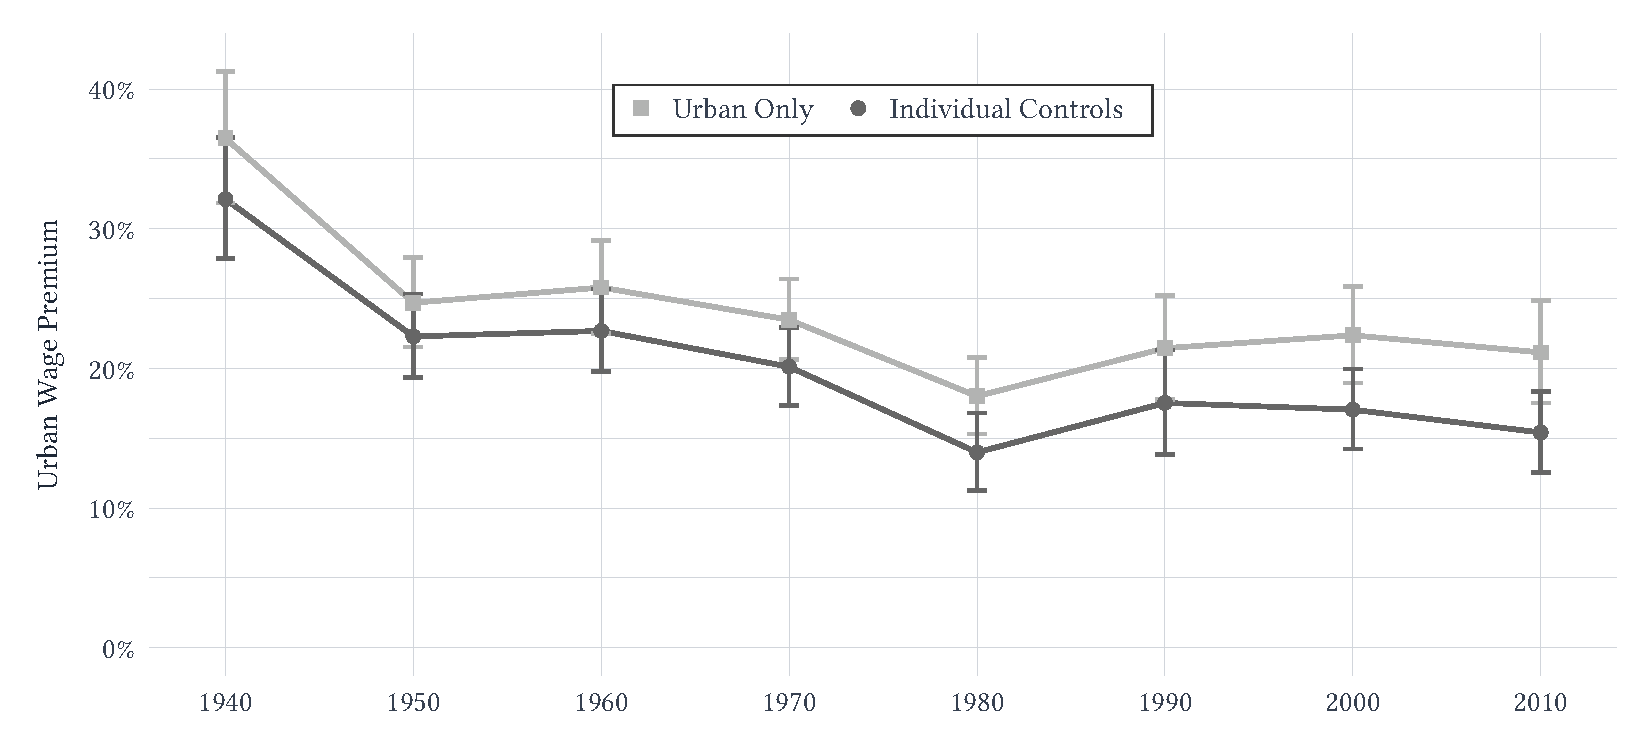
\includegraphics{figures/urban_premium/controls.pdf}
  \end{adjustbox}
  {\footnotesize\singlespacing
      \textit{Notes:} This figure plots the coefficient for survey-year level estimates of the urban wage premium from equation (\ref{eq:controls}) with different level of controls.
      The light gray line with square markers recreates the unadjusted point estimates.
      The dark gray line with circle markers includes controls for age in 5-year bins, education levels, and an indicator for being White.
      The points for each line are plotted with the 95 percent confidence intervals.
  }
\end{figure}
%%%%%%%%%%%%%%%%%

\clearpage\newpage

%%%%%%%%%%%%%%%%%
% Figure 2 %%%%%%
\begin{figure}[ht]
  \caption{Urban Wage Premium Controlling for Individual Characteristics and Sorting Using Group-Level Averages, 1940-2010}
  \label{fig:causal_premium}
  {\centering
      \resizebox{\columnwidth}{!}{
        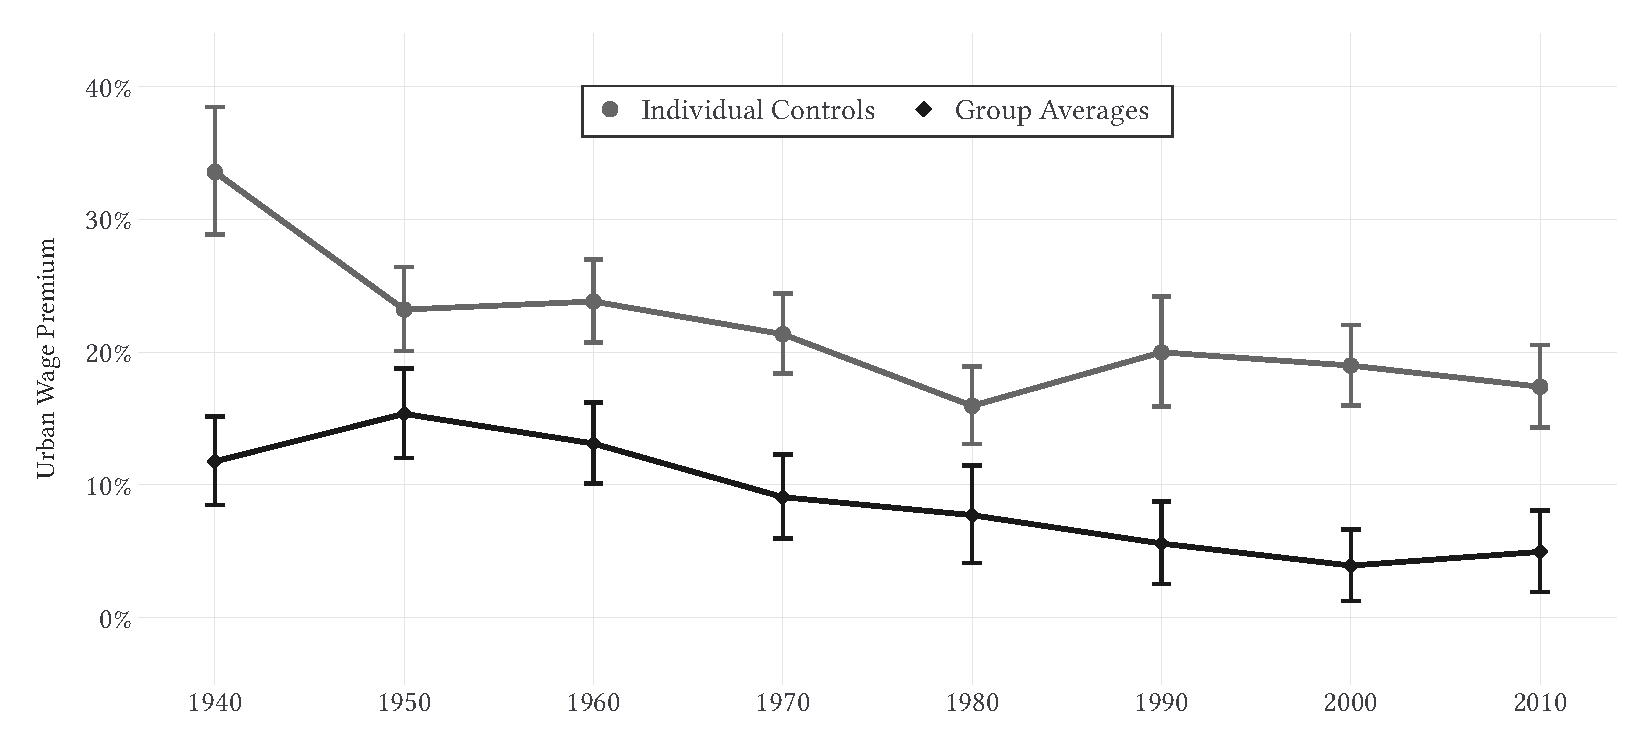
\includegraphics{figures/urban_premium/controls_and_causal.pdf}
      } 
  }%
  {\footnotesize\singlespacing
      \textit{Notes:} This figure plots the coefficient for survey-year level estimates of the urban wage premium following the methodology in Section \ref{sec:sorting}.
We estimate equation \eqref{eq:AM} with the individual-level and group-average controls.
These point estimates serve as our estimate for the causal urban wage premium. 
  }
\end{figure}
%%%%%%%%%%%%%%%%%%

\clearpage\newpage

%%%%%%%%%%%%%%%%%%
% Figure 3 %%%%%%%
\begin{figure}[ht]
  \caption{Urban Wage Premium Net of Housing Costs, 1940-2010}
  \begin{subfigure}{\linewidth}
    \caption{Raw Differences}
    \label{fig:raw_net_premium}
    \begin{adjustbox}{width=\textwidth,center}
      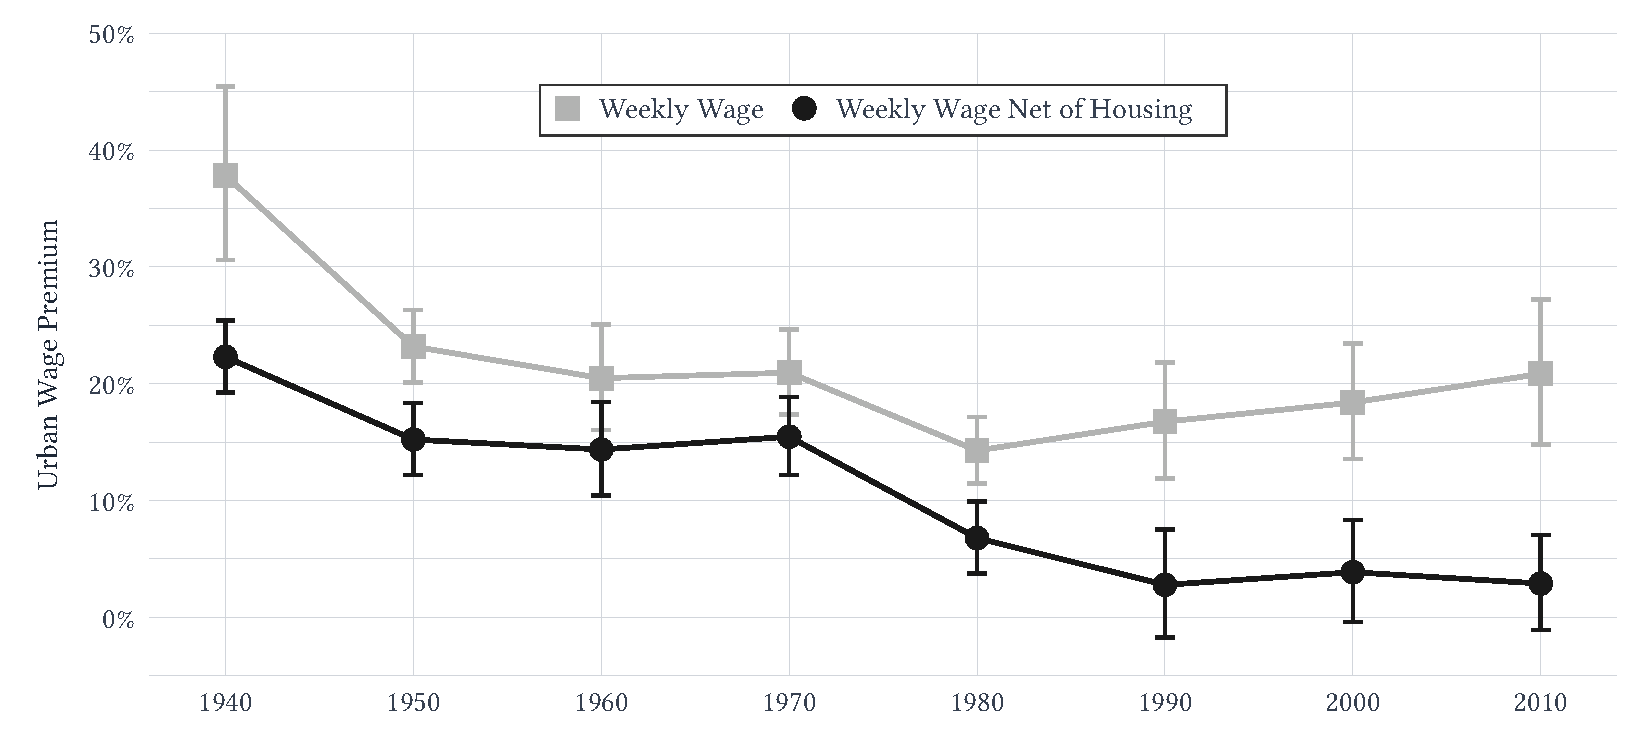
\includegraphics{figures/housing_costs/net_raw.pdf}
    \end{adjustbox}
  \end{subfigure}
  \begin{subfigure}{\linewidth}
    \caption{Controlling for Individual Characteristics and Sorting Using Group-Level Averages}
    \label{fig:causal_net_premium}
    \begin{adjustbox}{width=\textwidth,center}
      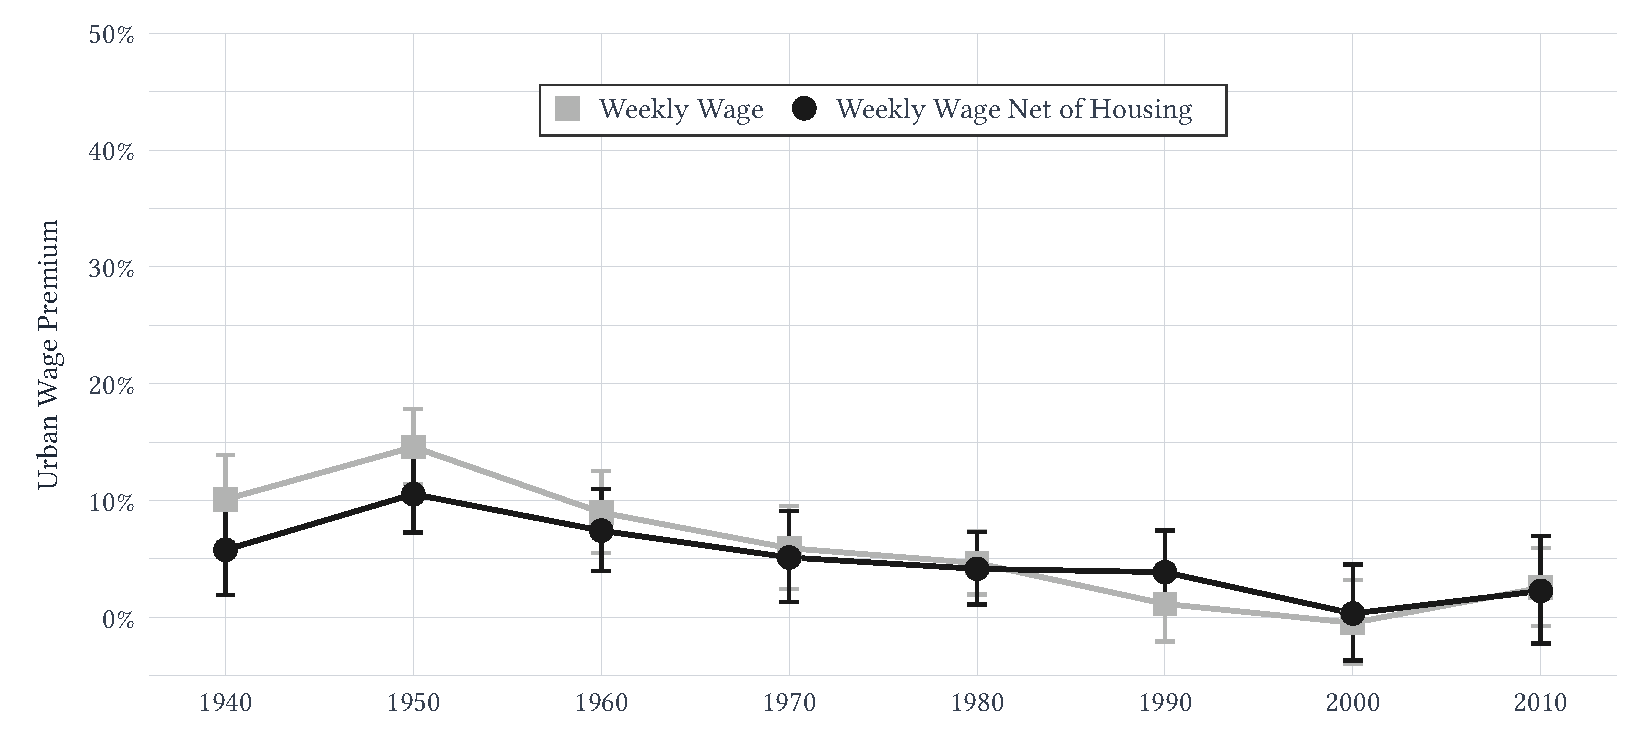
\includegraphics{figures/housing_costs/net_causal.pdf}
    \end{adjustbox}
  \end{subfigure}

  {\footnotesize\singlespacing
    \textit{Notes:} This figure recreates figures \ref{fig:premium_over_time} and \ref{fig:causal_premium} using a modified wage measure that subtracts off the cost of housing. 
  }
\end{figure}
%%%%%%%%%%%%%%%%%%%%%%

\clearpage\newpage
%%%%%%%%%%%%%%%%%
% Figure 4 %%%%%%
\begin{figure}[ht]
  \caption{Urban Wage Premium for Female Workers, 1940-2010}
  \label{fig:female_wage_premium}
  {\centering
    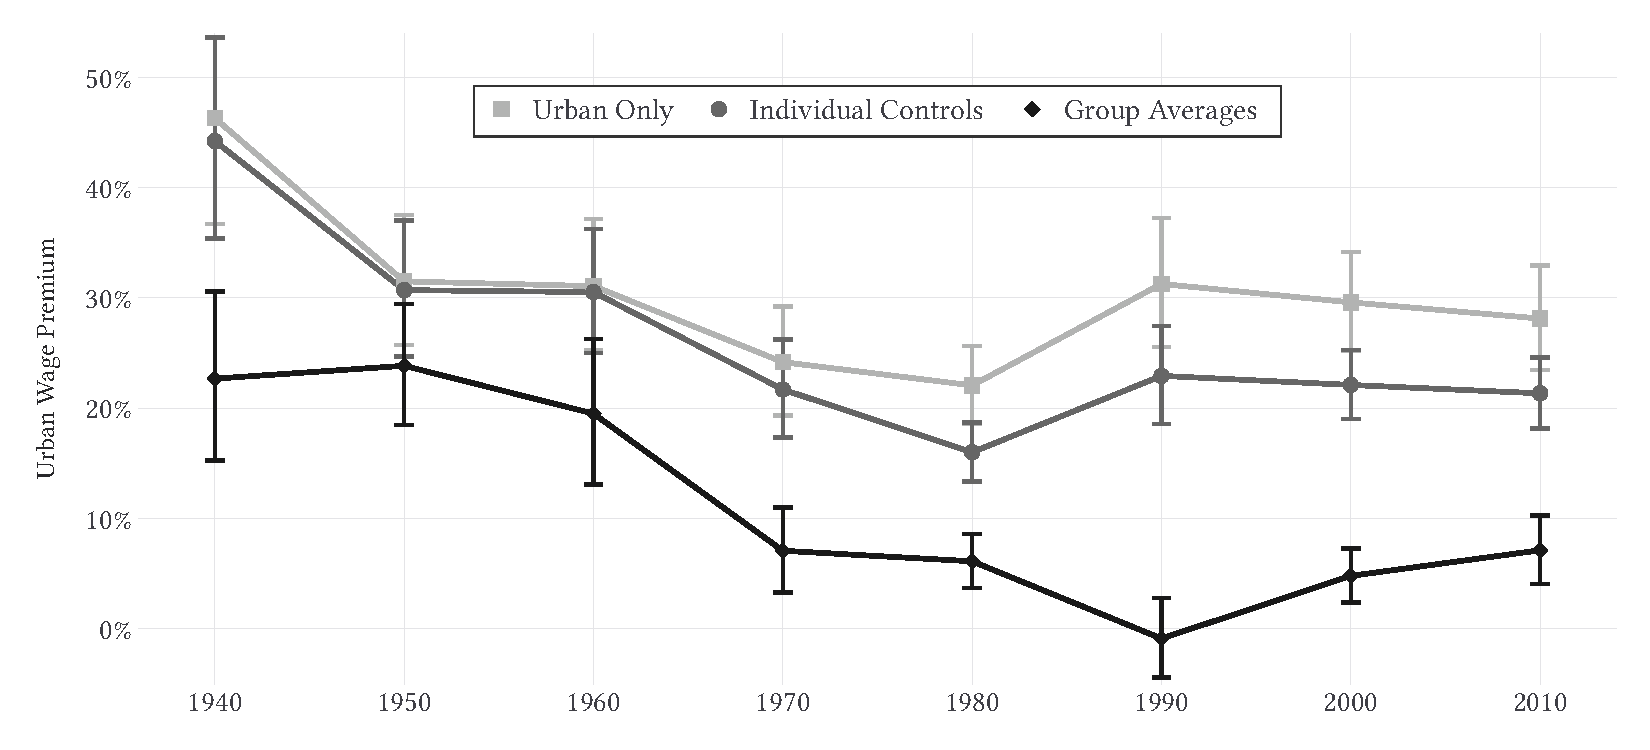
\includegraphics[width=\textwidth]{figures/female_urban_premium/combined.pdf}
  }

  {\footnotesize\singlespacing
      \textit{Notes:} This figure plots the coefficient for survey-year level estimates of the urban wage premium following the methodology in Section \ref{sec:sorting} using female workers instead of male workers.
  }
\end{figure}
%%%%%%%%%%%%


%%%%%%%%%%%%%%%%%
% Figure 5 %%%%%%
\begin{figure}[ht]
  \caption{Heterogeneity in Urban Wage Premium}\label{fig:heterogeneity}

  \vspace{2.5mm}
  \begin{subfigure}{\linewidth}
    \caption{City Size}
    {\centering
      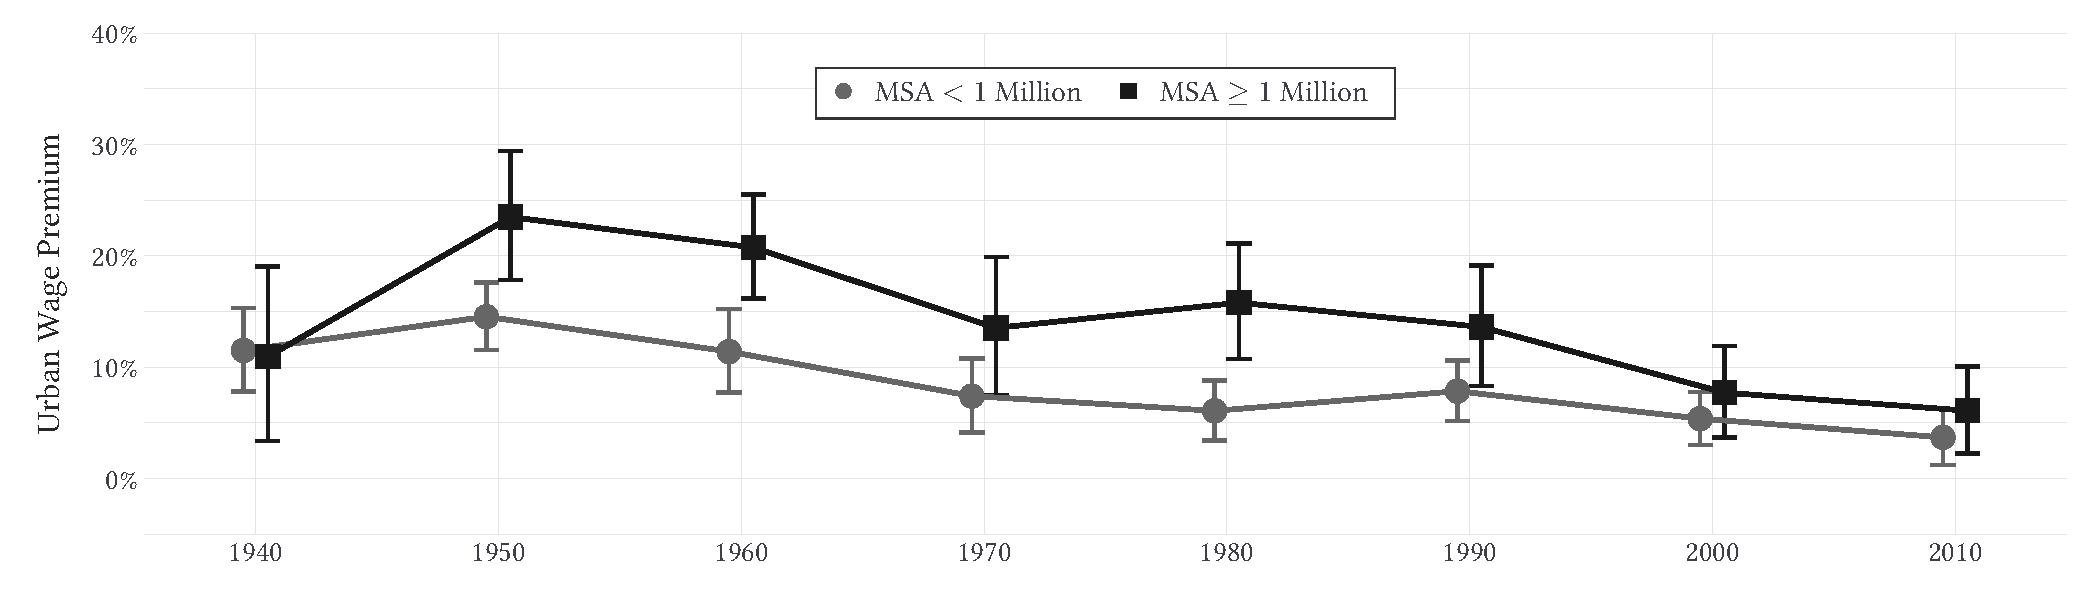
\includegraphics[width=\textwidth]{figures/heterogeneity/big_vs_small_cities.pdf}
    }
  \end{subfigure}

  \begin{subfigure}{\linewidth}
    \caption{Region}
    {\centering
      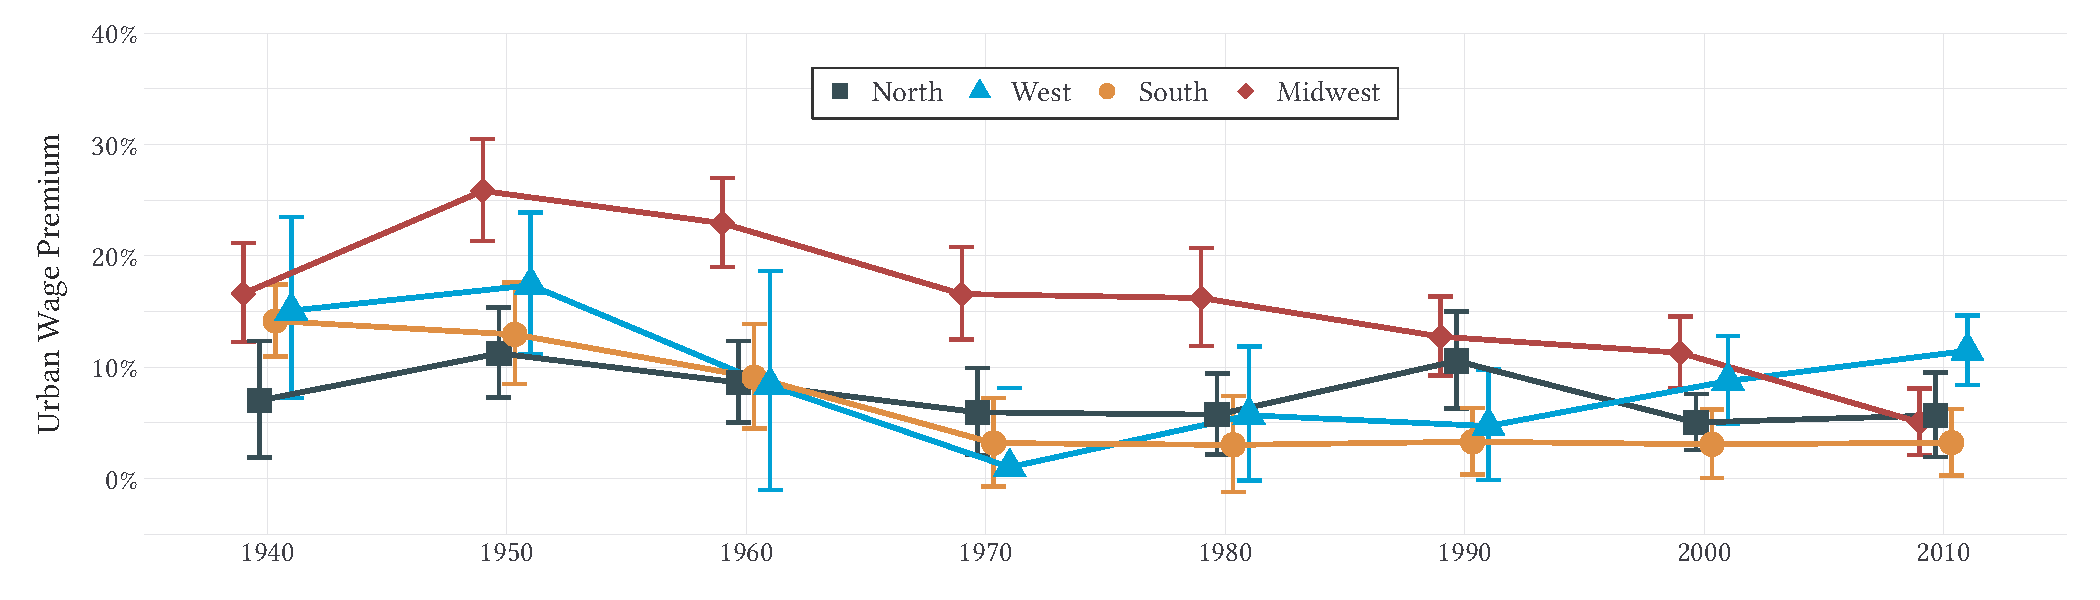
\includegraphics[width=\textwidth]{figures/heterogeneity/by_region.pdf}
    }
  \end{subfigure}

  \begin{subfigure}{\linewidth}
    \caption{Occupation}
    {\centering
      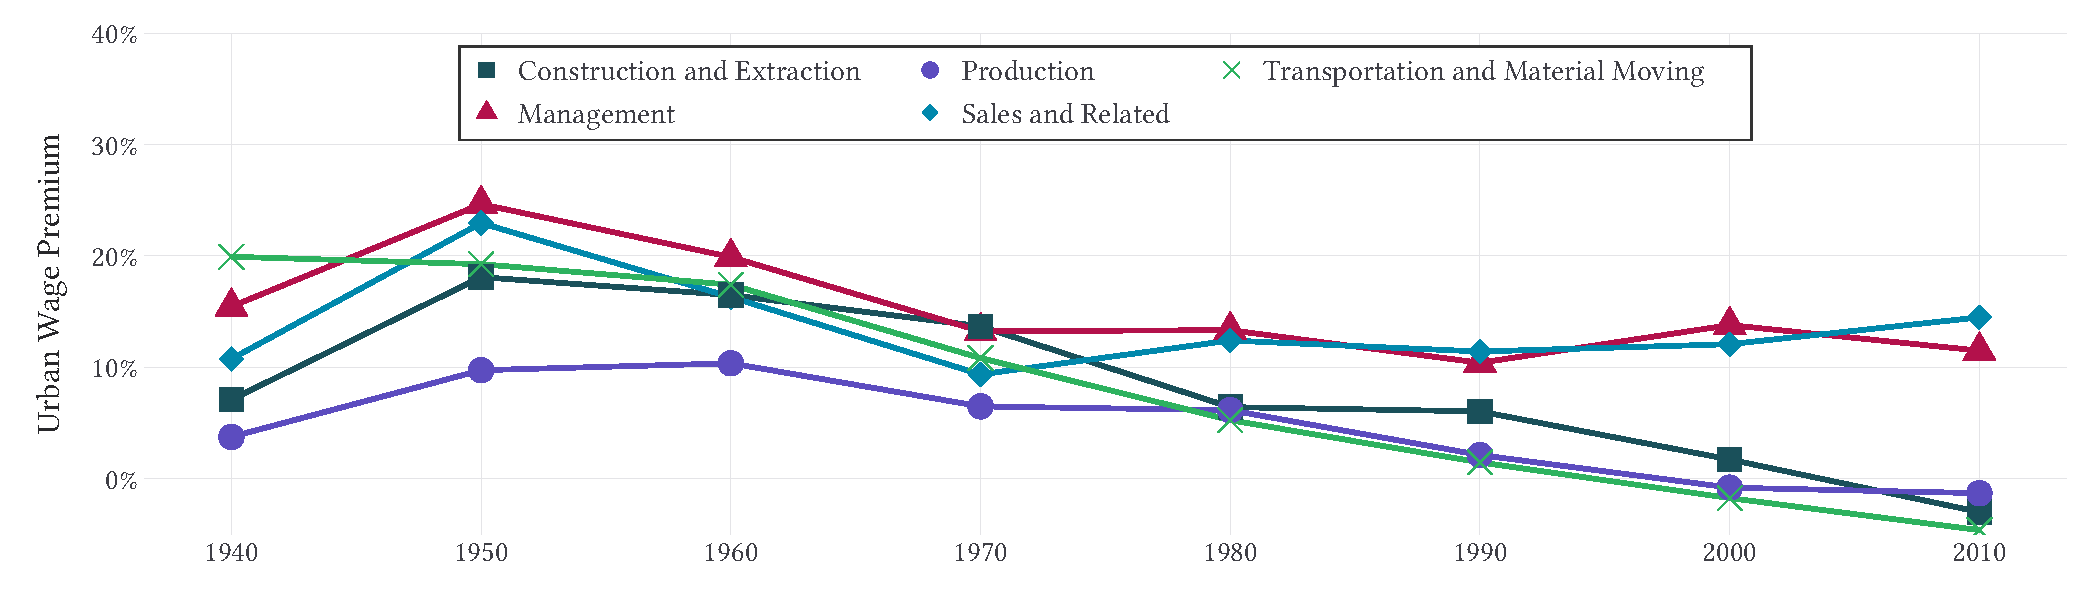
\includegraphics[width=\textwidth]{figures/heterogeneity/by_occupation.pdf}
    }
  \end{subfigure}

\end{figure}
%%%%%%%%%%%%%%%%%

\clearpage\newpage

%%%%%%%%%%%%%%%%%
% Figure 5 (cont.) %%%%%%
\begin{figure}[ht]\ContinuedFloat
  \caption{Heterogeneity in Urban Wage Premium (cont.)}

  \begin{subfigure}{\linewidth}
    \caption{Education}
    {\centering
      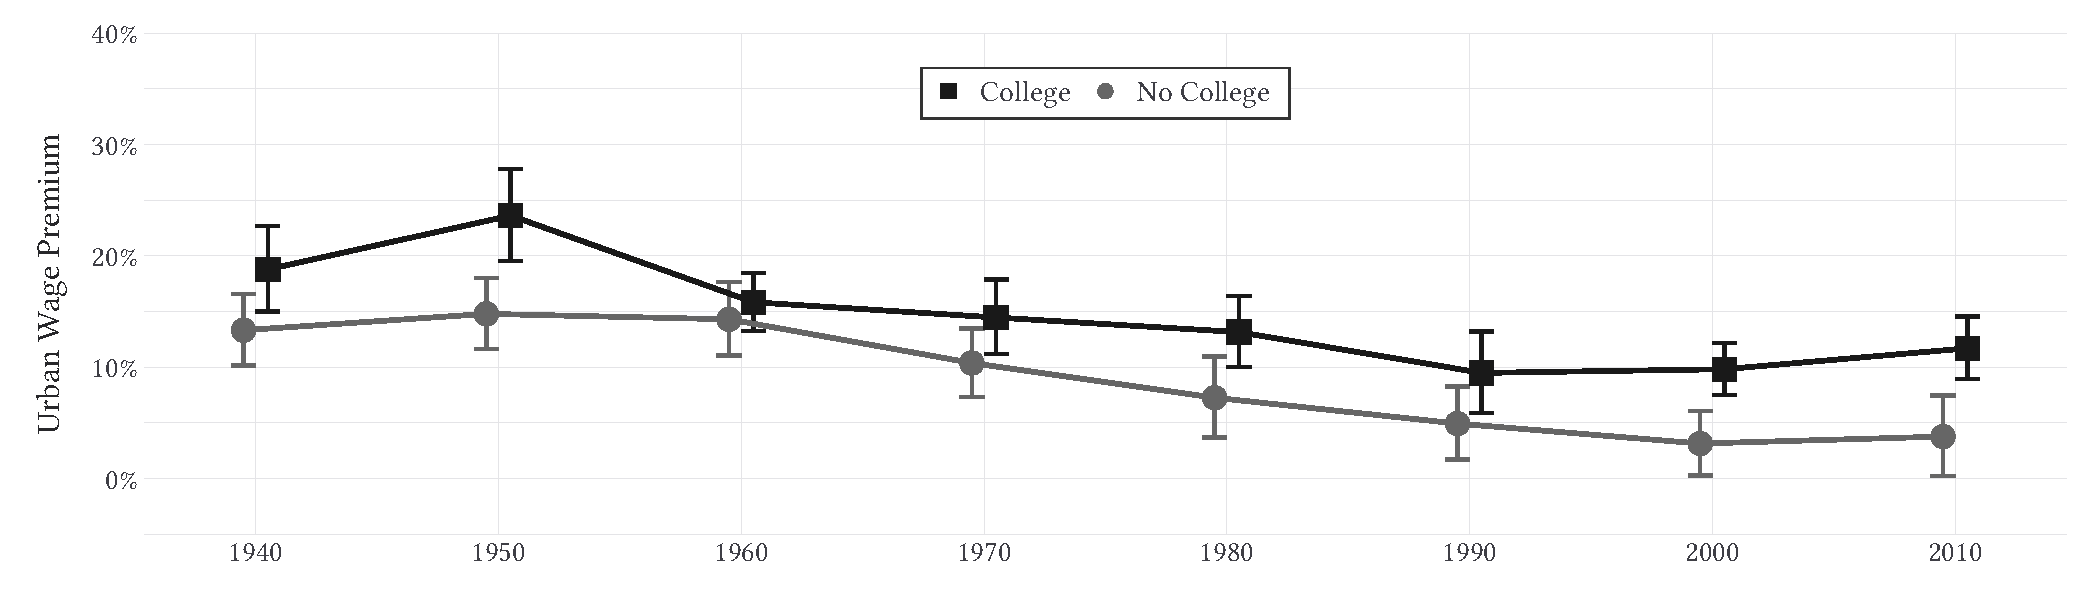
\includegraphics[width=\textwidth]{figures/heterogeneity/by_college.pdf}
    }
  \end{subfigure}

  \begin{subfigure}{\linewidth}
    \caption{Race}
    {\centering
      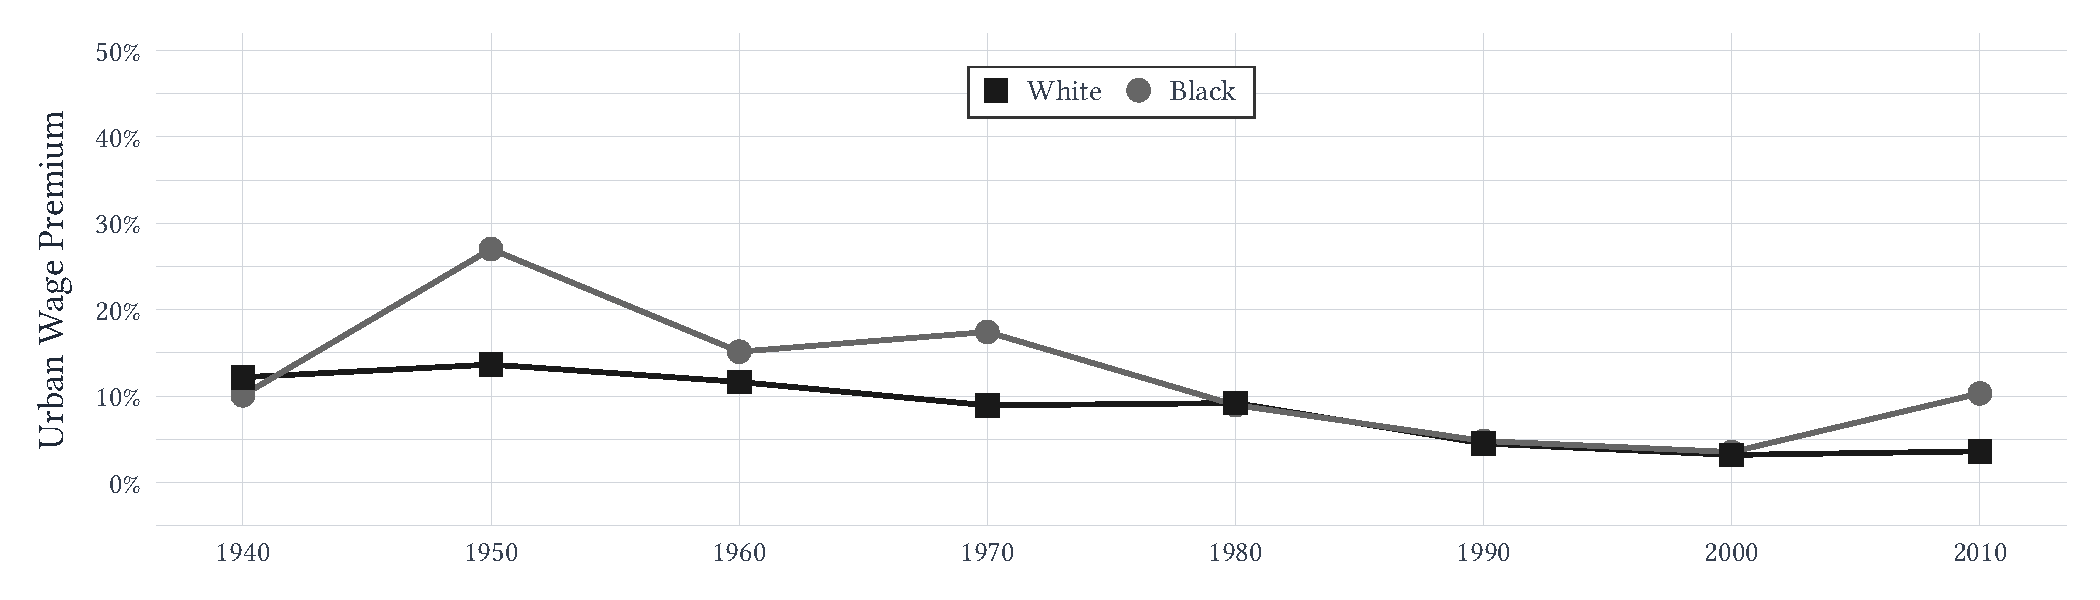
\includegraphics[width=\textwidth]{figures/heterogeneity/by_race.pdf}
    }
  \end{subfigure}

  \begin{subfigure}{\linewidth}
    \caption{Age}
    {\centering
      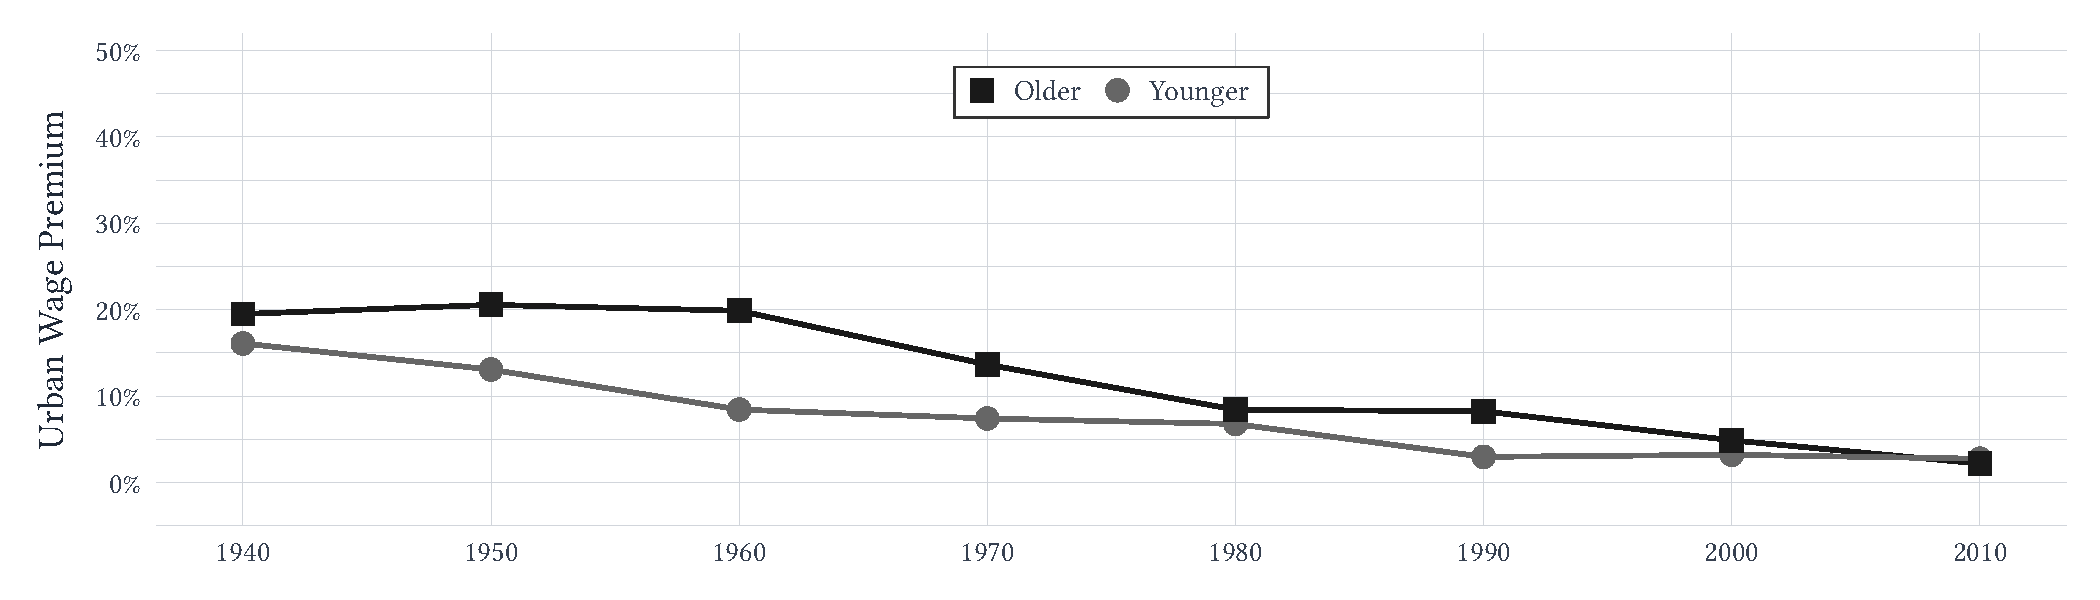
\includegraphics[width=\textwidth]{figures/heterogeneity/by_older.pdf}
    }
  \end{subfigure}

  \vspace{-5mm}
  {\footnotesize\singlespacing
      \textit{Notes:} This figure plots the coefficient for survey-year level estimates of the urban wage premium from equation (\ref{eq:AM}) including the individual-level and group-average controls described in section \ref{sec:sorting} while interacting urban status with various characteristics.  
      Panel A interacts the urban indicator with an indicator for the top 20 most populous MSA in 1940.
      Panel B interacts the urban indicator with indicators for each census region.
      Panel C interacts the urban indicator with indicators for each two-digit SOC industry code and presents estimates for the 5 largest industries in terms of employment.
      Panel D report estimates for separate samples of college- or non-college-educated workers.
      Panel E report estimates for separate samples of Black and White workers.
      Panel F\textbf{} report estimates for separate samples of college- or non-college-educated workers.
  }
\end{figure}
%%%%%%%%%%%%%%%%%

\clearpage\newpage

%%%%%%%%%%%%%%%%%%%%%%%%%%%%%%%%%%%%%%%%%%%%%%%%%%%%%%%%%%%

\newpage
\appendix 

\begin{center}
\hspace{0pt}
\vfill
\textbf{{\LARGE Online Appendix}}
\vfill
\hspace{0pt}
\end{center}

\numberwithin{equation}{section}
\numberwithin{figure}{section}
\numberwithin{table}{section}

\setcounter{figure}{0}
\renewcommand\thefigure{\Alph{section}\arabic{figure}}
\setcounter{table}{0}
\renewcommand\thetable{\Alph{section}\arabic{table}}

% ------------------------------------------------------------------------------


\newpage\clearpage

\section{Additional Tables and Figures}

\vspace{2in}


%%%%%%%%%%%%%%%%
\begin{table}[ht]
  \caption{Summary Statistics}
  \label{tab:summ}
  \renewcommand{\arraystretch}{1.25}

  \resizebox{\columnwidth}{!}{

  \begin{threeparttable}
    \begin{tabular}{@{} c @{\extracolsep{20pt}} c @{\extracolsep{5pt}} cccc @{}}
      % Head
      \toprule

      & & & \multicolumn{3}{c}{\% With College Degree} \\
      \cmidrule{4-6}
      Year & \multicolumn{1}{c}{\% Wage Gap} & \multicolumn{1}{c}{\% Urban} & \multicolumn{1}{c}{Overall} & \multicolumn{1}{c}{in Urban Areas} & \multicolumn{1}{c}{in Non-urban Areas} \\
      (1) & \multicolumn{1}{c}{(2)} & \multicolumn{1}{c}{(3)} & \multicolumn{1}{c}{(4)} & \multicolumn{1}{c}{(5)} & \multicolumn{1}{c}{(6)} \\  

      % Body
      \toprule

      1940 & 31.4 & 65.6 & 8.4 & 8.8 & 7.6 \\
1950 & 21.6 & 68.3 & 8.0 & 8.6 & 6.7 \\
1960 & 23.5 & 65.2 & 11.5 & 12.9 & 9.1 \\
1970 & 23.5 & 74.4 & 16.6 & 17.8 & 13.0 \\
1980 & 19.3 & 72.2 & 24.1 & 26.6 & 17.7 \\
1990 & 25.7 & 73.2 & 28.0 & 31.1 & 19.6 \\
2000 & 31.6 & 78.4 & 30.5 & 33.4 & 19.8 \\
2010 & 30.2 & 79.1 & 33.5 & 36.4 & 22.2 \\


      \bottomrule
    \end{tabular}
        
    % Notes 
    \begin{tablenotes}\footnotesize
        \item\noindent\textit{Notes.} This table presents summary statistics for the final ACS sample.
The data cleaning process is described in Section \ref{sec:data}.
    \end{tablenotes}
  \end{threeparttable}

  }
\end{table}
%%%%%%%%%%%

\newpage\clearpage

%%%%%%%%%%%%%%%%
\begin{table}[ht]
  \caption{Top Ten Cities by Urban Wage Premium in 1940 and 2010}
  \label{tab:top}
  \renewcommand{\arraystretch}{1.25}

  \resizebox{\columnwidth}{!}{
  \begin{threeparttable}
    \begin{tabular}{@{} lr @{\extracolsep{20pt}} l @{} r @{}}
      % Head
      \toprule

      \multicolumn{2}{c}{1940} & \multicolumn{2}{c}{2010} \\
      \cmidrule{1-2} \cmidrule{3-4} 
      Name & Premium & Name & Premium \\
        

      % Body
      \toprule

% Flint, MI & 47.9\% & San Jose-Sunnyvale-Santa Clara, CA & 63.2\% \\ 
% Detroit, MI & 46.0\% & Bridgeport-Stamford-Norwalk, CT & 54.7\% \\ 
% Washington DC, MD/VA/WV & 45.7\% & San Francisco-San Mateo-Redwood City,CA & 52.0\% \\ 
% San Francisco, CA & 44.0\% & Washington-Arlington-Alexandria DC-VA & 42.9\% \\ 
% Seattle-Everett, WA & 41.7\% & Boston-Quincy, MA & 42.7\% \\ 
% Lansing-East Lansing, MI & 41.0\% & Seattle-Bellevue-Everett, WA & 42.2\% \\ 
% New York, NY & 40.2\% & Santa Cruz-Watsonville, CA & 36.7\% \\ 
% Sacramento, CA & 39.2\% & Trenton-Ewing, NJ & 36.1\% \\ 
% Chicago, IL & 38.8\% & Midland, TX & 34.0\% \\ 
% Rochester, NY & 38.1\% & Baltimore-Towson, MD & 33.6\% \\ 

Flint, MI & 48.4\% & Stamford, CT & 80.5\% \\
Detroit, MI & 45.9\% & Danbury, CT & 56.9\% \\
San Francisco-Oakland-Vallejo, CA & 43.4\% & San Jose, CA & 51.5\% \\
Seattle-Everett, WA & 42.6\% & Washington, DC/MD/VA & 46.5\% \\
Washington, DC/MD/VA & 42.3\% & Monmouth-Ocean, NJ & 45.5\% \\
Lansing-East Lansing, MI & 38.8\% & Boston, MA& 41.5\% \\
Sacramento, CA & 38.6\% & Trenton, NJ & 41.3\% \\
New York, NY & 38.4\% & Bridgeport, CT & 41.2\% \\
Milwaukee, WI & 38.1\% & San Francisco, CA & 39.6\% \\
Rochester, NY & 38.1\% & Nashua, NH & 37.7\% \\
    

      \bottomrule
    \end{tabular}
        
    % Notes 
    \begin{tablenotes}\footnotesize
        \item \textit{Notes.} This table presents the top ten cities in terms of observed wage premia relative to non-urban areas.
    \end{tablenotes}
  \end{threeparttable}
  }

\end{table}
%%%%%%%%%%%

\newpage\clearpage

%%%%%%%%%%%%%%%%
\begin{table}[ht]
  \caption{Estimates of the Urban Wage Premium, 1940-2010}
  \label{tab:wage_premium}
  \renewcommand{\arraystretch}{1.25}

  \resizebox{\columnwidth}{!}{
  \begin{threeparttable}
    \begin{tabular}{@{} l *{8}{c} @{}}
      % Head
      \toprule

      & \multicolumn{8}{c}{$\log(\text{Weekly Wage})$}\\
      \cmidrule{2-9}
      
      & 1940 & 1950 & 1960 & 1970 & 1980 & 1990 & 2000 & 2010 \\
        

      % Body
      \toprule
      
\multicolumn{9}{l}{\hspace{-2.5mm}{\bfseries \itshape Panel A: Raw Wage Premium}} \\
$\text{Urban} = 1$ & 0.3162$^{***}$ & 0.2208$^{***}$ & 0.2288$^{***}$ & 0.2109$^{***}$ & 0.1692$^{***}$ & 0.1939$^{***}$ & 0.2014$^{***}$ & 0.1898$^{***}$\\
& (0.0192) & (0.0131) & (0.0134) & (0.0119) & (0.0110) & (0.0158) & (0.0144) & (0.0155)\\
\midrule

\multicolumn{9}{l}{\hspace{-2.5mm}{\bfseries \itshape Panel B: Individual Controls}} \\
$\text{Urban} = 1$ & 0.2822$^{***}$ & 0.2012$^{***}$ & 0.2038$^{***}$ & 0.1833$^{***}$ & 0.1334$^{***}$ & 0.1609$^{***}$ & 0.1566$^{***}$ & 0.1414$^{***}$\\
& (0.0186) & (0.0125) & (0.0123) & (0.0119) & (0.0116) & (0.0163) & (0.0125) & (0.0127)\\
\midrule

\multicolumn{9}{l}{\hspace{-2.5mm}{\bfseries \itshape Panel C: Individual Controls \& Group Averages}} \\
$\text{Urban} = 1$ & 0.1216$^{***}$ & 0.1506$^{***}$ & 0.1251$^{***}$ & 0.0883$^{***}$ & 0.0731$^{***}$ & 0.0487$^{***}$ & 0.0359$^{***}$ & 0.0499$^{***}$\\
& (0.0144) & (0.0167) & (0.0144) & (0.0154) & (0.0171) & (0.0160) & (0.0137) & (0.0147)\\
\midrule

Observations & 2,504,957 & 68,457 & 1,364,524 & 280,338 & 1,907,943 & 2,260,990 & 2,582,144 & 2,718,970\\

      \bottomrule
    \end{tabular}
        
    % Notes 
    \begin{tablenotes}[flushleft]\footnotesize
        \item\textit{Notes.} This table reports coefficient for survey-year level estimates of the urban wage premium from equation (\ref{eq:controls}) with three different level of controls.
The first section includes no controls and represents the urban wage premium observed in the data.
The second section includes controls for age in 5-year bins, education levels, and an indicator for being White.
The final section includes group-average variables following the methodology in Section \ref{sec:sorting}.
These point estimates serve as our estimate for the causal urban wage premium.
        
        \item Signif.
Codes: $^{***}$: 0.01, $^{**}$: 0.05, $^{*}$: 0.1.
Standard errors are clustered  by MSA/CBSA.
    \end{tablenotes}
  \end{threeparttable}
  }

\end{table}
%%%%%%%%%%%

\newpage\clearpage

%%%%%%%%%%%%%%%%
\begin{table}[ht]
  \caption{Heterogeneity in the Urban Wage Premium, 1940-2010}
  \label{tab:heterogeneity}
  \renewcommand{\arraystretch}{1.25}

  \resizebox{\columnwidth}{!}{
  \begin{threeparttable}
    \begin{tabular}{@{} l *{8}{c} @{}}
      % Head
      \toprule

      % & \multicolumn{8}{c}{$\log(\text{Weekly Wage})$}\\
      % \cmidrule{2-9}
      
      & 1940 & 1950 & 1960 & 1970 & 1980 & 1990 & 2000 & 2010 \\
        

      % Body
      \toprule

      
\multicolumn{9}{l}{\hspace{-2.5mm}{\bfseries \itshape Panel A: Big vs. Small Cities}} \\

MSA $< 1$ Million & 0.111$^{***}$ & 0.137$^{***}$ & 0.105$^{***}$ & 0.071$^{***}$ & 0.058$^{***}$ & 0.076$^{***}$ & 0.051$^{***}$ & 0.036$^{***}$ \\
  & (0.02) & (0.01) & (0.02) & (0.02) & (0.01) & (0.01) & (0.01) & (0.01) \\
MSA $\geq 1$ Million & 0.114$^{***}$ & 0.214$^{***}$ & 0.189$^{***}$ & 0.127$^{***}$ & 0.146$^{***}$ & 0.129$^{***}$ & 0.076$^{***}$ & 0.060$^{***}$ \\
  & (0.04) & (0.02) & (0.02) & (0.03) & (0.02) & (0.02) & (0.02) & (0.02) \\


\midrule

\multicolumn{9}{l}{\hspace{-2.5mm}{\bfseries \itshape Panel B: By Region}} \\

North & 0.068$^{***}$ & 0.106$^{***}$ & 0.083$^{***}$ & 0.058$^{***}$ & 0.056$^{***}$ & 0.100$^{***}$ & 0.049$^{***}$ & 0.055$^{***}$ \\
  & (0.02) & (0.02) & (0.02) & (0.02) & (0.02) & (0.02) & (0.01) & (0.02) \\
West & 0.140$^{***}$ & 0.160$^{***}$ & 0.080$^{*}$ & 0.010 & 0.055$^{*}$ & 0.046$^{*}$ & 0.084$^{***}$ & 0.109$^{***}$ \\
  & (0.04) & (0.03) & (0.05) & (0.03) & (0.03) & (0.02) & (0.02) & (0.01) \\
South & 0.132$^{***}$ & 0.122$^{***}$ & 0.087$^{***}$ & 0.031 & 0.030 & 0.032$^{**}$ & 0.030$^{**}$ & 0.032$^{**}$ \\
  & (0.01) & (0.02) & (0.02) & (0.02) & (0.02) & (0.01) & (0.02) & (0.01) \\
Midwest & 0.154$^{***}$ & 0.230$^{***}$ & 0.206$^{***}$ & 0.153$^{***}$ & 0.150$^{***}$ & 0.120$^{***}$ & 0.107$^{***}$ & 0.049$^{***}$ \\
  & (0.02) & (0.02) & (0.02) & (0.02) & (0.02) & (0.02) & (0.01) & (0.01) \\


\midrule

\multicolumn{9}{l}{\hspace{-2.5mm}{\bfseries \itshape Panel D: Education}} \\

College & 0.172$^{***}$ & 0.212$^{***}$ & 0.147$^{***}$ & 0.135$^{***}$ & 0.123$^{***}$ & 0.091$^{***}$ & 0.094$^{***}$ & 0.111$^{***}$ \\
  & (0.02) & (0.02) & (0.01) & (0.01) & (0.01) & (0.02) & (0.01) & (0.01) \\
No College & 0.125$^{***}$ & 0.138$^{***}$ & 0.134$^{***}$ & 0.099$^{***}$ & 0.070$^{***}$ & 0.048$^{***}$ & 0.031$^{**}$ & 0.037$^{**}$ \\
  & (0.01) & (0.01) & (0.01) & (0.01) & (0.02) & (0.02) & (0.01) & (0.02) \\


\midrule

\multicolumn{9}{l}{\hspace{-2.5mm}{\bfseries \itshape Panel C: Race}} \\

White & 0.110$^{***}$ & 0.127$^{***}$ & 0.112$^{***}$ & 0.087$^{***}$ & 0.089$^{***}$ & 0.046$^{***}$ & 0.033$^{**}$ & 0.036$^{**}$ \\
  & (0.02) & (0.01) & (0.02) & (0.02) & (0.02) & (0.01) & (0.02) & (0.02) \\
Black & 0.089$^{***}$ & 0.237$^{***}$ & 0.139$^{***}$ & 0.160$^{***}$ & 0.085$^{***}$ & 0.048$^{**}$ & 0.036$^{**}$ & 0.098$^{***}$ \\
  & (0.03) & (0.03) & (0.02) & (0.03) & (0.02) & (0.02) & (0.02) & (0.02) \\


\midrule

\multicolumn{9}{l}{\hspace{-2.5mm}{\bfseries \itshape Panel E: Age}} \\

Older & 0.183$^{***}$ & 0.187$^{***}$ & 0.181$^{***}$ & 0.128$^{***}$ & 0.081$^{***}$ & 0.079$^{***}$ & 0.048$^{***}$ & 0.022 \\
  & (0.02) & (0.02) & (0.01) & (0.01) & (0.02) & (0.01) & (0.01) & (0.01) \\
Younger & 0.146$^{***}$ & 0.123$^{***}$ & 0.081$^{***}$ & 0.072$^{***}$ & 0.066$^{***}$ & 0.029$^{*}$ & 0.032$^{**}$ & 0.027$^{*}$ \\
  & (0.02) & (0.01) & (0.02) & (0.01) & (0.02) & (0.02) & (0.02) & (0.01) \\



      \bottomrule
    \end{tabular}
        
    % Notes 
    \begin{tablenotes}[flushleft]\footnotesize
        \item\textit{Notes.} This table reports coefficient and standard errors corresponding to Figures \ref{fig:heterogeneity}.
        
        \item Signif.
Codes: $^{***}$: 0.01, $^{**}$: 0.05, $^{*}$: 0.1.
Standard errors are clustered  by MSA/CBSA.
    \end{tablenotes}
  \end{threeparttable}
  }

\end{table}
%%%%%%%%%%%

\newpage\clearpage

%%%%%%%%%%%%%%%%
\begin{table}[ht]
  \caption{Industry-Specific Urban Wage Premium Estimates, 1940-2010}
  \label{tab:industry_specific}
  \renewcommand{\arraystretch}{1.25}

  \resizebox{\columnwidth}{!}{
  \begin{threeparttable}
    \begin{tabular}{@{} l *{8}{c} @{}}
      % Head
      \toprule

      % & \multicolumn{8}{c}{$\log(\text{Weekly Wage})$}\\
      % \cmidrule{2-9}
      
      & 1940 & 1950 & 1960 & 1970 & 1980 & 1990 & 2000 & 2010 \\
        
      % Body
      \toprule


Management & 0.142$^{***}$ & 0.213$^{***}$ & 0.183$^{***}$ & 0.126$^{***}$ & 0.126$^{***}$ & 0.100$^{***}$ & 0.131$^{***}$ & 0.110$^{***}$ \\
  & (0.02) & (0.02) & (0.02) & (0.02) & (0.02) & (0.01) & (0.01) & (0.02) \\
Business and Financial Operations & 0.117$^{***}$ & 0.184$^{***}$ & 0.087$^{***}$ & 0.058$^{***}$ & 0.098$^{***}$ & 0.084$^{***}$ & 0.123$^{***}$ & 0.169$^{***}$ \\
  & (0.02) & (0.03) & (0.01) & (0.02) & (0.02) & (0.02) & (0.02) & (0.02) \\
Architecture and Engineering & 0.079$^{***}$ & 0.094$^{***}$ & 0.037$^{***}$ & 0.034$^{**}$ & 0.037$^{**}$ & 0.012 & 0.054$^{***}$ & 0.060$^{***}$ \\
  & (0.02) & (0.03) & (0.01) & (0.02) & (0.02) & (0.01) & (0.01) & (0.02) \\
Life, Physical, and Social Science & 0.030$^{*}$ & 0.065$^{**}$ & 0.060$^{***}$ & 0.089$^{***}$ & 0.030 & -0.008 & 0.007 & 0.127$^{***}$ \\
  & (0.02) & (0.03) & (0.01) & (0.02) & (0.02) & (0.01) & (0.02) & (0.02) \\
Community and Social Services & 0.096$^{***}$ & 0.053 & 0.046$^{**}$ & 0.047$^{**}$ & 0.125$^{***}$ & 0.092$^{***}$ & 0.072$^{***}$ & 0.100$^{***}$ \\
  & (0.02) & (0.05) & (0.02) & (0.02) & (0.02) & (0.02) & (0.01) & (0.02) \\
Education, Training, and Library & 0.101$^{***}$ & 0.113$^{***}$ & 0.049$^{***}$ & 0.024 & 0.040$^{***}$ & -0.019 & -0.010 & 0.026 \\
  & (0.02) & (0.03) & (0.02) & (0.02) & (0.02) & (0.01) & (0.01) & (0.02) \\
Arts, Design, Entertainment, Sports, and Media & 0.126$^{***}$ & 0.087$^{**}$ & 0.119$^{***}$ & 0.138$^{***}$ & 0.161$^{***}$ & 0.145$^{***}$ & 0.149$^{***}$ & 0.129$^{***}$ \\
  & (0.02) & (0.04) & (0.02) & (0.03) & (0.03) & (0.02) & (0.03) & (0.03) \\
Healthcare Practitioners and Technical & -0.125 & -0.057 & -0.106 & -0.021 & 0.055$^{***}$ & 0.026 & 0.021 & 0.040$^{**}$ \\
  & (0.02) & (0.06) & (0.02) & (0.02) & (0.02) & (0.02) & (0.01) & (0.02) \\
Healthcare Support & -0.029 & -0.030 & 0.071$^{***}$ & 0.016 & 0.098$^{***}$ & 0.090$^{***}$ & 0.064$^{***}$ & 0.118$^{***}$ \\
  & (0.02) & (0.05) & (0.02) & (0.05) & (0.03) & (0.02) & (0.02) & (0.02) \\
Protective Service & 0.165$^{***}$ & 0.136$^{***}$ & 0.127$^{***}$ & 0.124$^{***}$ & 0.136$^{***}$ & 0.101$^{***}$ & 0.099$^{***}$ & 0.083$^{***}$ \\
  & (0.03) & (0.02) & (0.02) & (0.02) & (0.02) & (0.02) & (0.02) & (0.02) \\
Food Preparation and Serving Related & 0.074$^{***}$ & 0.143$^{***}$ & 0.148$^{***}$ & 0.063$^{***}$ & 0.085$^{***}$ & 0.091$^{***}$ & 0.083$^{***}$ & 0.167$^{***}$ \\
  & (0.02) & (0.02) & (0.02) & (0.02) & (0.02) & (0.02) & (0.02) & (0.02) \\
Building and Grounds Cleaning and Maintenance & 0.128$^{***}$ & 0.105$^{***}$ & 0.184$^{***}$ & 0.113$^{***}$ & 0.054$^{***}$ & 0.039$^{**}$ & 0.062$^{***}$ & 0.099$^{***}$ \\
  & (0.02) & (0.03) & (0.02) & (0.02) & (0.02) & (0.02) & (0.02) & (0.02) \\
Personal Care and Service & 0.148$^{***}$ & 0.198$^{***}$ & 0.176$^{***}$ & 0.073$^{***}$ & 0.122$^{***}$ & 0.122$^{***}$ & 0.043 & 0.107$^{***}$ \\
  & (0.02) & (0.03) & (0.01) & (0.02) & (0.03) & (0.03) & (0.03) & (0.03) \\
Sales and Related & 0.100$^{***}$ & 0.208$^{***}$ & 0.154$^{***}$ & 0.091$^{***}$ & 0.118$^{***}$ & 0.109$^{***}$ & 0.116$^{***}$ & 0.137$^{***}$ \\
  & (0.02) & (0.02) & (0.02) & (0.02) & (0.02) & (0.01) & (0.01) & (0.02) \\
Office and Administrative Support & -0.016 & 0.029$^{*}$ & 0.041$^{***}$ & 0.024$^{*}$ & 0.023 & -0.003 & 0.015 & 0.048$^{***}$ \\
  & (0.02) & (0.02) & (0.01) & (0.01) & (0.02) & (0.01) & (0.01) & (0.02) \\
Farming, Fishing, and Forestry & 0.208$^{***}$ & 0.240$^{***}$ & 0.246$^{***}$ & -0.012 & 0.092 & 0.018 & -0.089 & -0.108 \\
  & (0.02) & (0.08) & (0.07) & (0.08) & (0.06) & (0.04) & (0.02) & (0.03) \\
Construction and Extraction & 0.069$^{***}$ & 0.167$^{***}$ & 0.156$^{***}$ & 0.130$^{***}$ & 0.065$^{***}$ & 0.060$^{***}$ & 0.018 & -0.030 \\
  & (0.02) & (0.02) & (0.02) & (0.02) & (0.02) & (0.02) & (0.02) & (0.02) \\
Installation, Maintenance, and Repair & 0.066$^{***}$ & 0.103$^{***}$ & 0.096$^{***}$ & 0.083$^{***}$ & 0.062$^{***}$ & 0.045$^{***}$ & 0.018 & -0.000 \\
  & (0.02) & (0.02) & (0.01) & (0.02) & (0.02) & (0.02) & (0.01) & (0.01) \\
Production & 0.036$^{**}$ & 0.093$^{***}$ & 0.101$^{***}$ & 0.064$^{***}$ & 0.061$^{***}$ & 0.022 & -0.007 & -0.013 \\
  & (0.02) & (0.02) & (0.01) & (0.02) & (0.02) & (0.02) & (0.02) & (0.01) \\
Transportation and Material Moving & 0.183$^{***}$ & 0.179$^{***}$ & 0.164$^{***}$ & 0.104$^{***}$ & 0.053$^{***}$ & 0.015 & -0.017 & -0.047 \\
  & (0.02) & (0.02) & (0.02) & (0.02) & (0.02) & (0.01) & (0.01) & (0.02) \\


      \bottomrule
    \end{tabular}
        
    % Notes 
    \begin{tablenotes}[flushleft]\footnotesize
        \item\textit{Notes.} This table reports coefficient and standard errors corresponding to Figures \ref{fig:heterogeneity}.
        
        \item Signif.
Codes: $^{***}$: 0.01, $^{**}$: 0.05, $^{*}$: 0.1.
Standard errors are clustered  by MSA/CBSA.
    \end{tablenotes}
  \end{threeparttable}
  }

\end{table}
%%%%%%%%%%%

\newpage\clearpage

%%%%%%%%%%%%%%%%%
\begin{figure}[ht]
  \caption{Urban Wage Premium Using the 1940 Definition of MSAs, 1940-2010}
  \label{fig:premium_msa_in_all_yrs}
  {\centering
    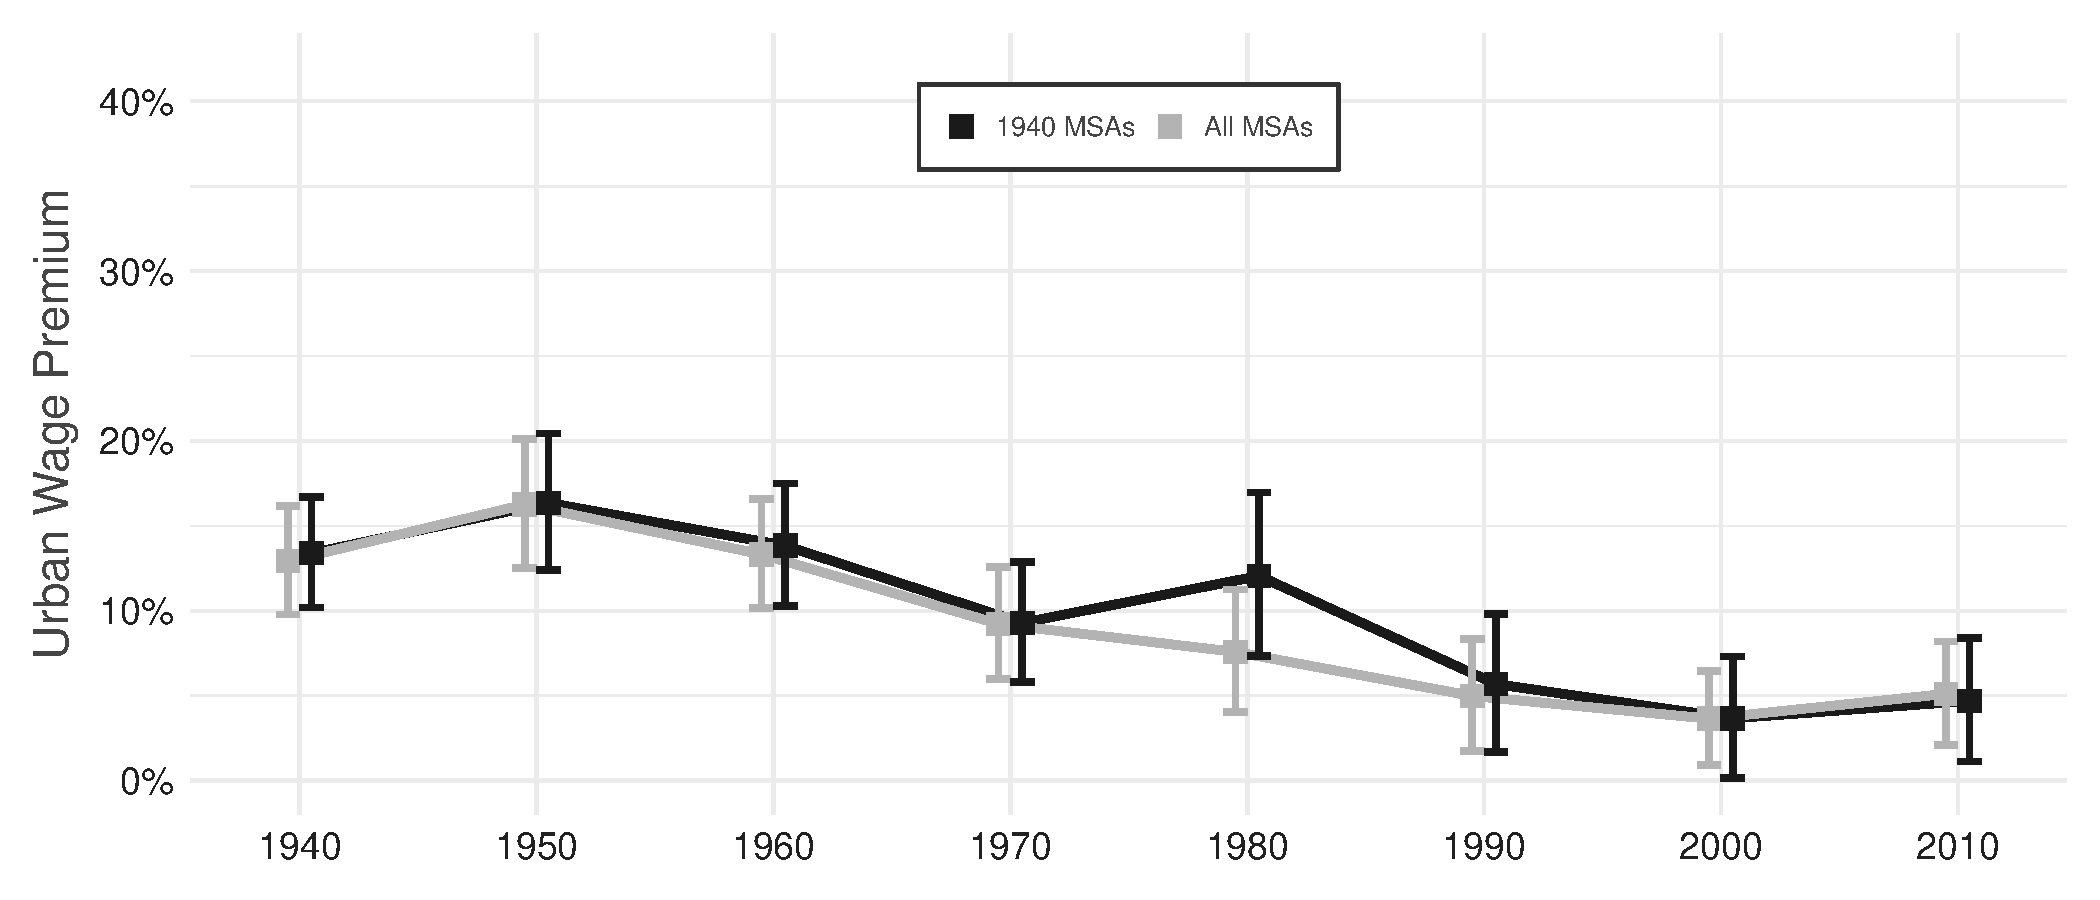
\includegraphics[width=\textwidth]{figures/urban_premium/1940_msas_compared.pdf}
  }

  {\footnotesize\singlespacing
      \textit{Notes:} This figure plots the coefficient for survey-year level estimates of the urban wage premium following the methodology in Section \ref{sec:sorting}.
We estimate equation \eqref{eq:AM} with the individual-level and group-average controls using only the subsample of 1940 MSAs.
Individuals living in MSAs that were added after 1940 are dropped from the sample.
The estimates from Figure \ref{fig:causal_premium} are reproduced for comparison.
  }
\end{figure}
%%%%%%%%%%%%

\newpage\clearpage

%%%%%%%%%%%%%%%%%
\begin{figure}[ht]
  \caption{Urban Wage Premium Using only Full-Time Workers, 1940-2010}
  \label{fig:premium_full_time_employees}
  {\centering
    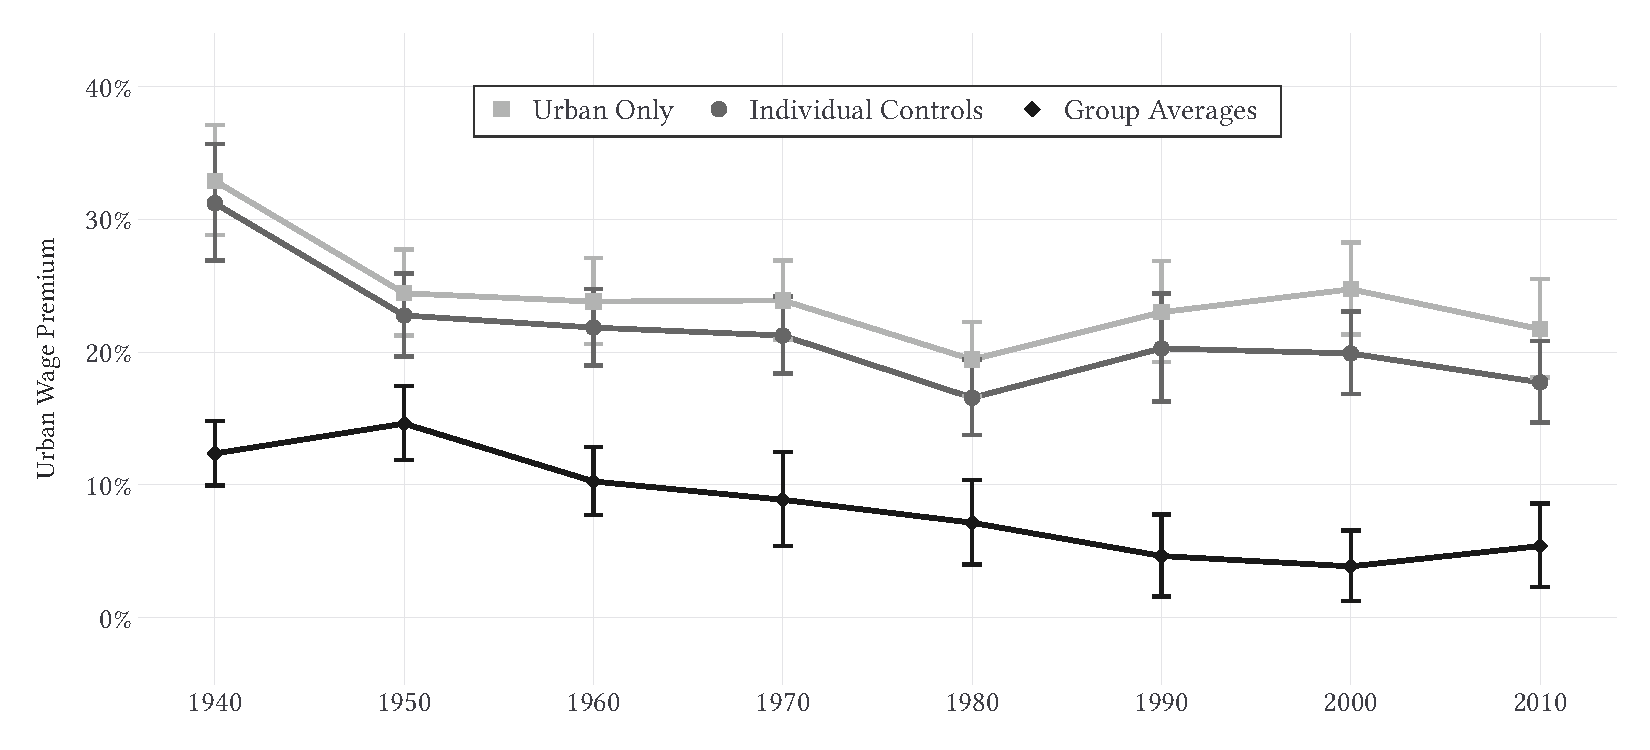
\includegraphics[width=\textwidth]{figures/robustness/urban_premium_full_time_employees.pdf}
  }

  {\footnotesize\singlespacing
    \textit{Notes:} This figure plots the coefficient for survey-year level estimates of the urban wage premium following the methodology in Section \ref{sec:sorting}.
    Individuals who work less than 51 weeks are dropped from the sample.
  }
\end{figure}
%%%%%%%%%%%%


\newpage\clearpage

%%%%%%%%%%%%%%%%%
\begin{figure}[ht]
  \caption{Leave One Location Average Out Estimates}
  \label{fig:leave_one_group_average_out}
  {\centering
    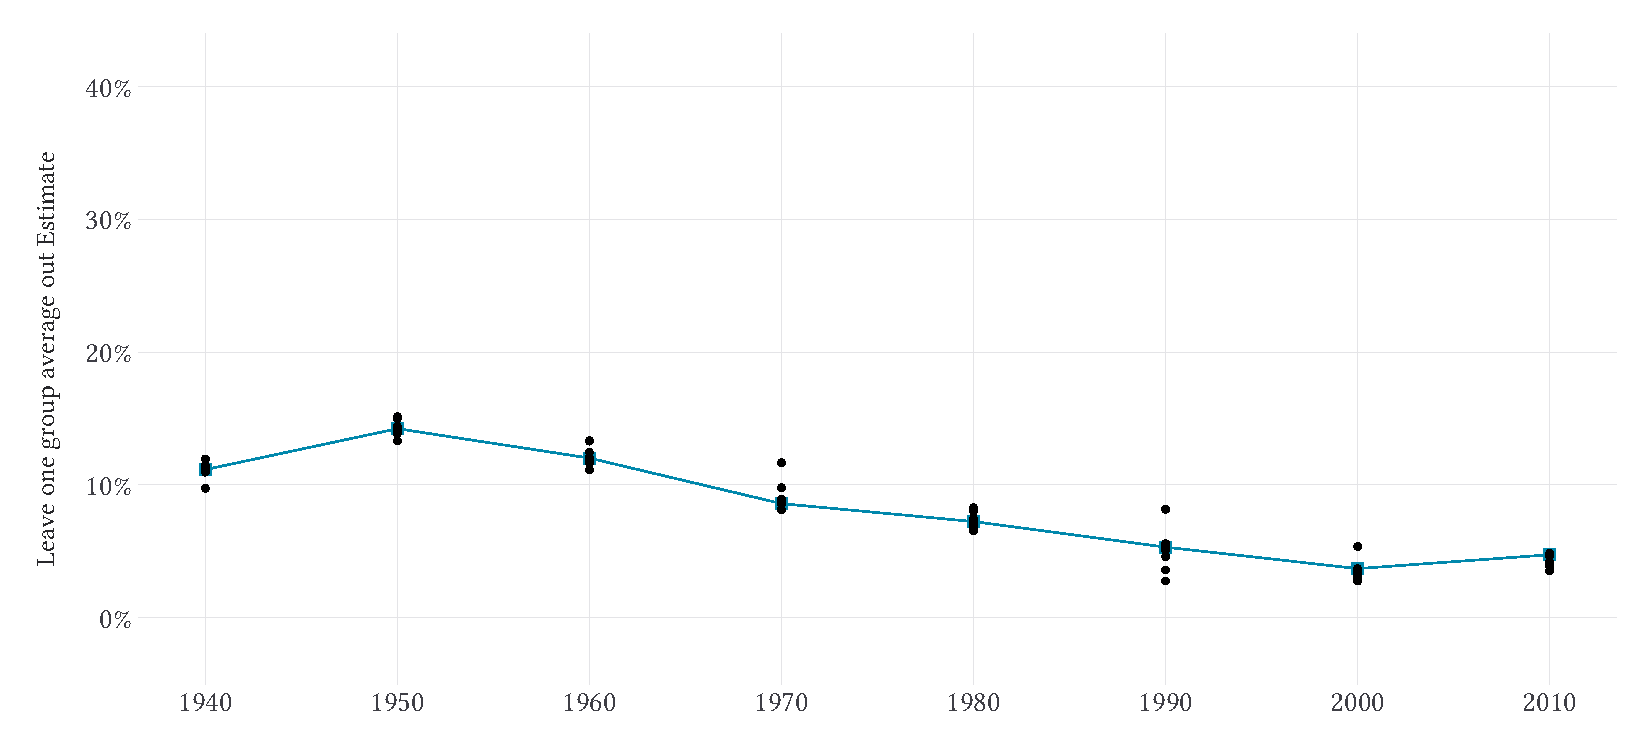
\includegraphics[width=\textwidth]{figures/robustness/leave_one_group_average_out.pdf}
  }

  {\footnotesize\singlespacing
    \textit{Notes:} This figure plots the coefficient for survey-year level estimates of the urban wage premium following the methodology in Section \ref{sec:sorting}.
    The connected line represents the original estimates while the black circles correspond to estimates that leave one of the location-averages out of the regression. 
  }
\end{figure}
%%%%%%%%%%%%


\newpage\clearpage

%%%%%%%%%%%%%%%%%
\begin{figure}[ht]
  \caption{Distribution of Wage Residuals, 1940-2010}
  \label{fig:9010}

  \vspace{5mm}
  \begin{subfigure}{\linewidth}
    \caption{Aggregate Distribution}
    {\centering
      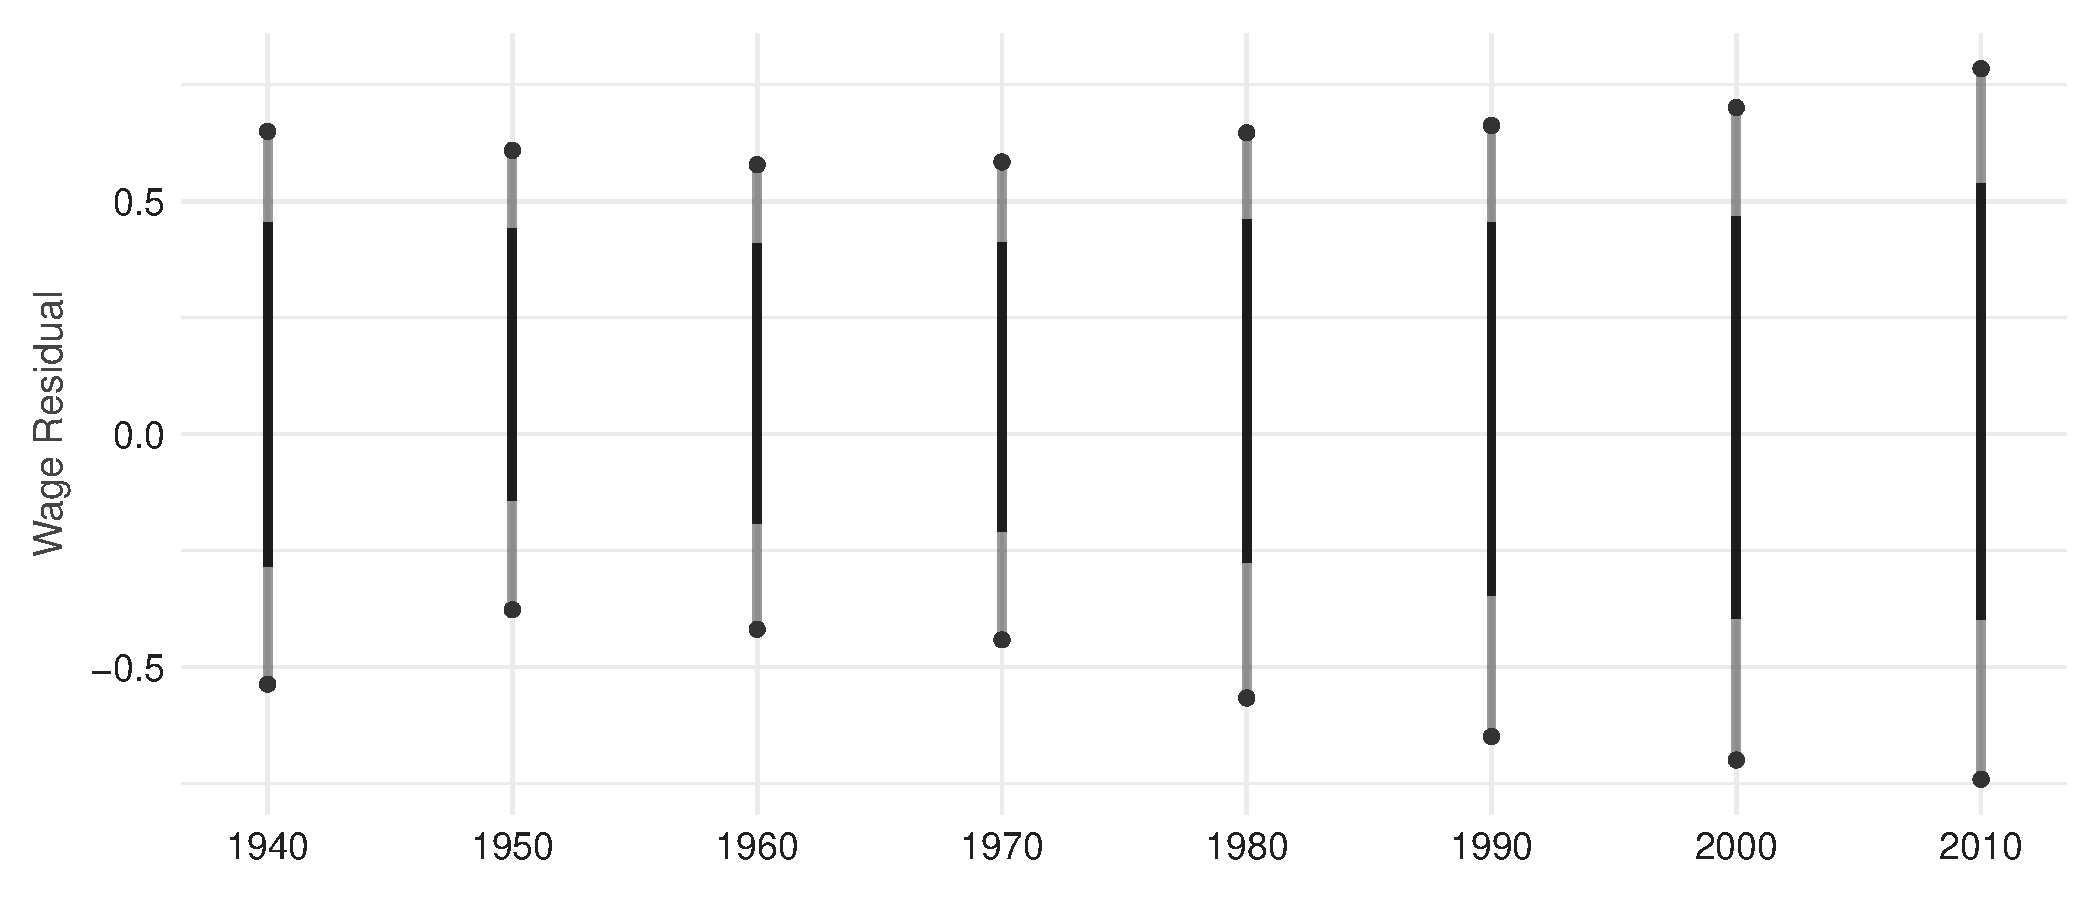
\includegraphics[width=\linewidth]{figures/distribution/9010.pdf}
    }
  \end{subfigure}

  \begin{subfigure}{\linewidth}
    \caption{Urban versus Non-urban Distribution}
    {\centering
      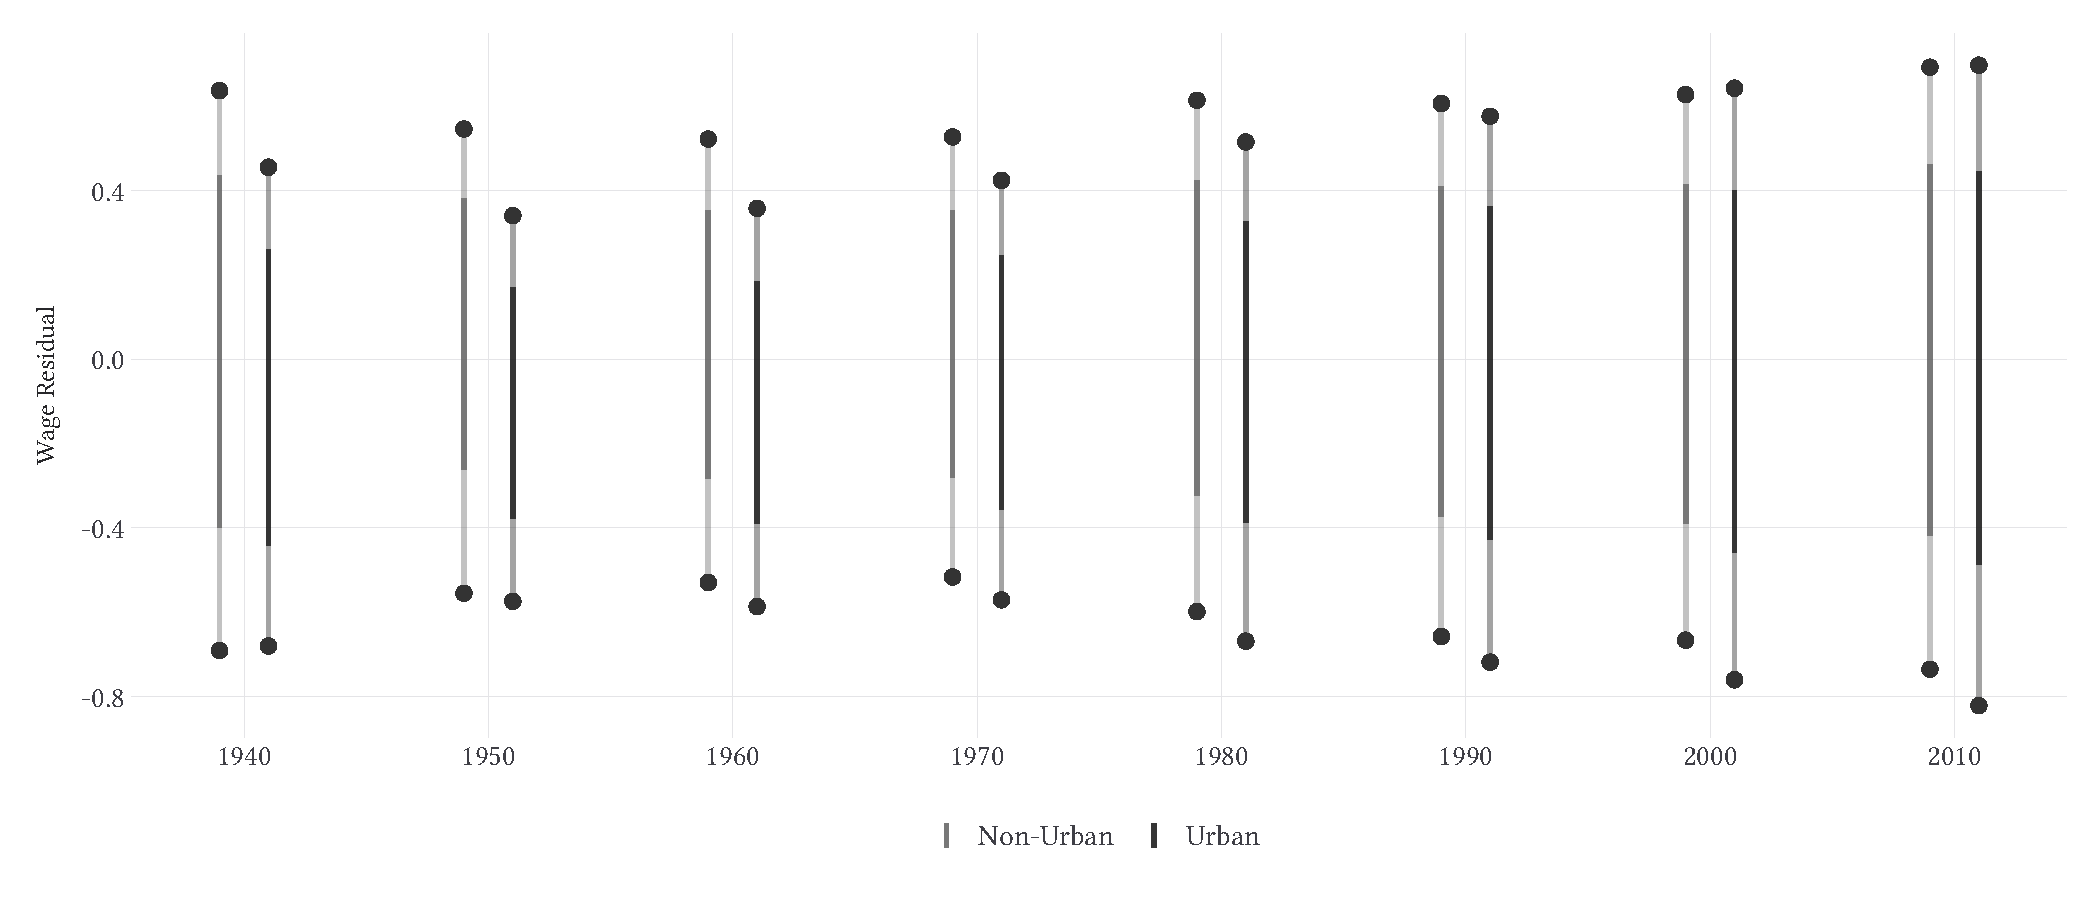
\includegraphics[width=\linewidth]{figures/distribution/9010_urban.pdf}
    }
  \end{subfigure}

  \vspace{-7.5mm}
  {\footnotesize\singlespacing
      \textit{Notes:} This figure takes the residual of wages after regressing on the full-specification and adds back in the causal urban wage premium.
Each panel plots points for the 90th-10th percentiles of the wage residuals and shades darker the 80th-20th percentiles.
Panel A does this for the entire distribution of wages following \citet{goldin1992great}.
Panel B does this separately for urban and non-urban workers.
  }
\end{figure}
%%%%%%%%%%%%

\end{document}


%\begin{figure}
%  \caption{The Urban Rent Premium, 1940-2010}
%  \label{fig:premium_over_time}
%  {\centering
%      \resizebox{\columnwidth}{!}{
%          \includegraphics{figures/rentpremium_urban.pdf}
%      } 
%  }%
%  {\footnotesize\singlespacing
%      \textit{Notes:} This figure plots the coefficient for survey-year level estimates of the urban rent premium from equation (\ref{eq:controls}) without covariates and replacing the log weekly wage with log monthly gross rent.
% The points for each line are plotted with the 95 percent confidence intervals.
%  }
%\end{figure}


\subsection{Distributional Estimates}

In the period after World War II, there were substantial changes in wage inequality. 
\citet{goldin1992great} discuss the narrowing of the wage distribution in what they label the ``Great Compression'' between 1940 and 1960.
They highlight the rapid increase in the supply increase of educated workers during a period of relatively stagnant demand growth.
Recently, \citet{vickers2021effects} discuss the role of the National War Labor Board on wages in various regions throughout the country and show that wage-setting policies had a meaningful impact on local wage distributions. 


To explore whether we observe a compression and then widening of the wage distribution in our setting, we take the residuals from \eqref{eq:AM} which reflect individual earnings after controlling for sorting.
The ninetieth-tenth percentiles summarize the distribution of the wage residuals for each decade in Panel A of Figure \ref{fig:9010}.
Similar to \citet{goldin1992great}, we find evidence consistent with a narrowing of the wage distribution through 1960.
Afterward, the wage distribution widens considerably through 2010.

In Panel B of Figure \ref{fig:9010}, we plot the distribution of residuals for urban and non-urban workers.
In 1940, urban and non-urban workers had a large left tail in the wage distribution, reflecting many workers who earned very low (residualized) weekly earnings.
Between 1940 and 1960 this left-tail disappeared, which provides some evidence that a rising floor potentially drove the Great Compression on non-urban wages.\footnote{
The overall compression and the narrowing of the left-tail are also apparent when using $95^{th}$ and $5^{th}$ percentiles.} \citet{goldin1992great} find similar evidence that increases in the distribution for low-wage workers drove the Great Compression.
Our estimates suggest that the narrowing of the wage distribution occurred in urban and non-urban areas.



\clearpage\newpage

%%%%%%%%%%%%%%%%%
% Short Version %%%%%%
\begin{longtblr}[
    caption={Comparable Estimates in Literature},
    label = {tblr:estimates-in-literature},
    note{}={\vspace{-8mm}\footnotesize\singlespacing\textit{Notes:} 
      This table presents estimates of urban wage premium from other papers that use \emph{individual fixed-effects}. 
      It is not intended to be a complete collection.
      Papers that estimate wage premium as a function of population density were not included as we can not directly compare results.
    },
]{
  width=\textwidth,
  colspec = {X[2,l] X[2,l] X[r]},
} 

\toprule
\textbf{Reference} & & \textbf{Estimate} \\ 
\midrule 

%% Table 1 column (3)
\citet{BaumSnow_Pavan_2012}, NLSY 1990s
& $\hookrightarrow$ MSA $>$ 1.5Mill & 15\% \\ 
& $\hookrightarrow$ MSA 250K -- 1.5Mill  & 7\% \\[2ex]

%% Table 3 columns (8) and (9)
\citet{Glaeser_Mare_2001}, NLSY (1990s) and PSID (1990s) 
& $\hookrightarrow$ MSA $>$ 500k & 10.9\%, 4.5\% \\[2ex]

%% Table 2 column (7)
\citet{Yankow_2006}, NLSY 1990s 
& $\hookrightarrow$ MSA $>$ 1Mill & 5\% \\ 
& $\hookrightarrow$ MSA 250K -- 1Mill  & 3.3\% \\[2ex]

%% Table 2 column (3)
\citet{DCosta_Overman_2014}, 
& $\hookrightarrow$ Overall & 2.3\% \\ 
UK ASHE Survey 1998 -- 2008  & & \\[2ex]

%% Table 2 column (3) and Table 3 column (5) and (6)
\citet{carlsen2016education}, & $\hookrightarrow$ Oslo & 6.5\% \\
Norway Administrative data (2000s) & $\hookrightarrow$ Six other large cities & 4.5\% \\[2ex]

%% Table 2
\citet{donovan2024unraveling}, Meta-Analysis
& $\hookrightarrow$ Average of 160 panel data estimates & 5.8\% \\[2ex]

%% Table 6
\citet{ahlfeldt2019economic}, Meta-Analysis 
& $\hookrightarrow$ High-income countries & $\approx$ 4\% \\
& $\hookrightarrow$ Non-high-income countries & $\approx$ 8\% \\

\bottomrule
\end{longtblr}
%%%%%%%%%%%%%%%%%


\clearpage\newpage

%%%%%%%%%%%%%%%%%
% Long Version %%%%%%
\begin{longtblr}[ 
caption={Comparable Estimates in Literature},
label = {tblr:estimates-in-literature},
note{}={\vspace{-8mm}\footnotesize\singlespacing\textit{Notes:} 
  This table presents estimates of urban wage premium from other papers that use \emph{individual fixed-effects}. 
  It is not intended to be a complete collection.
  Papers that estimate wage premium as a function of population density were not included as we can not directly compare results.
},
]                     %% tabularray outer close
{                     %% tabularray inner open
  width=\textwidth,
  % colspec={Q[]Q[]Q[]Q[]},
  colspec = {X[2.5,l] X[2.5,l] X[r]},
}                     %% tabularray inner close

\toprule
\textbf{Reference} & \textbf{Estimate} \\ \midrule 

%% Table 1 column (3)
\citet{BaumSnow_Pavan_2012}, NLSY (1990s) & & \\ 
& $\hookrightarrow$ MSA $>$ 1.5Mill & 15\% \\ 
  & \hspace{5mm} $\hookrightarrow$ College & 6\% \\
  & \hspace{5mm} $\hookrightarrow$ Non-college & 18\% \\[2ex]
& $\hookrightarrow$ MSA 250K -- 1.5Mill  & 7\% \\[2ex]
  & \hspace{5mm} $\hookrightarrow$ College & 7\% \\
  & \hspace{5mm} $\hookrightarrow$ Non-college & 3.7\% \\[2ex]

%% Table 3 columns (8) and (9)
\citet{Glaeser_Mare_2001} & 1990s & NLSY  &  \\
& $\hookrightarrow$ MSA $>$ 500k & 10.9\% \\[2ex]

& 1990s & PSID  &  \\
& $\hookrightarrow$ MSA $>$ 500k & 4.5\% \\[2ex]

%% Table 2 column (7)
\citet{Yankow_2006} & 1990s & NLSY & \\ 
& $\hookrightarrow$ MSA $>$ 1Mill & 5\% \\ 
& $\hookrightarrow$ MSA 250K -- 1Mill  & 3.3\% \\[2ex]

%% Table 2 column (3)
\citet{DCosta_Overman_2014} & 1998 -- 2008 & UK ASHE Survey & \\
& $\hookrightarrow$ Overall & 2.3\% \\
  & \hspace{5mm} $\hookrightarrow$ London & 7.1\% \\
  & \hspace{5mm} $\hookrightarrow$ `Big City' & 2.5\% \\
  & \hspace{5mm} $\hookrightarrow$ `Small City' & 1.4\% \\[2ex]

%% Table 2 column (3) and Table 3 column (5) and (6)
\citet{carlsen2016education} & 2000s & Norway Administrative data & \\
& $\hookrightarrow$ Oslo & 6.5\% \\
  & \hspace{5mm} $\hookrightarrow$ College & 7.6\% \\
  & \hspace{5mm} $\hookrightarrow$ Non-college & 5\% \\[2ex]
& $\hookrightarrow$ Six other large cities & 4.5\% \\
  & \hspace{5mm} $\hookrightarrow$ College & 5.1\% \\
  & \hspace{5mm} $\hookrightarrow$ Non-college & 3.7\% \\[2ex]

%% Table 2
\citet{donovan2024unraveling} & 1980s -- 2010s & Meta-Analysis of `Agglomeration Elasticities' & \\
& $\hookrightarrow$ Average over 160 studies using panel data & 5.8\% \\[2ex]

%% Table 6
\citet{ahlfeldt2019economic} & 1980s -- 2010s & Meta-Analysis of `Agglomeration Elasticities' &  \\
& $\hookrightarrow$ High-income countries & $\approx$ 4\% \\
& $\hookrightarrow$ Non-high-income countries & $\approx$ 8\% \\[2ex]
\bottomrule
\end{longtblr}
%%%%%%%%%%%%%%%%%
